\documentclass{article}
\usepackage[fleqn]{amsmath}
\usepackage{amssymb,graphicx,color,graphicx,slashed, microtype, parskip, enumitem, extarrows, needspace}
%\usepackage[utf8x]{inputenc}
\usepackage[top=1.5cm, bottom=1.5cm, right=6cm, left=1.5cm, heightrounded, marginparwidth=5cm, marginparsep=0.5cm]{geometry}

\hbadness = 10000
\hfuzz=100pt 
    
\usepackage{marginnote}
\renewcommand*{\marginfont}{\footnotesize}

\usepackage{hyperref}
\hypersetup{colorlinks=true, urlcolor=NavyBlue, bookmarksdepth=3}

\makeatletter\newcommand{\@minipagerestore}{\setlength{\parskip}{\medskipamount}}\makeatother

% =============== Index ===========================

\usepackage[nonewpage]{imakeidx}
\makeindex

% =============== Color Definitions ===============
    
\usepackage[svgnames]{xcolor}
\colorlet{ColorTitle}{Black}
\colorlet{ColorSectionName}{Black}
\colorlet{ColorBoxFG}{Gray}
\colorlet{ColorBoxText}{Black}
\colorlet{ColorBoxBG}{White}


% =============== Title Style ===============
    
\usepackage{titling} % Allows custom title configuration
    
\newcommand{\HorRule}{\color{ColorTitle}\rule{\linewidth}{1pt}} % Defines the gold horizontal rule around the title
    
\pretitle{
    \vspace{-50pt} % Move the entire title section up
    \HorRule\vspace{9pt} % Horizontal rule before the title
    \fontsize{27}{36}\usefont{OT1}{phv}{b}{n}\selectfont
    \color{ColorTitle} % Text colour for the title and author(s)
}
    
\posttitle{\par\vskip 15pt} % Whitespace under the title
    
\preauthor{\fontsize{17}{0}\usefont{OT1}{phv}{m}{n}\selectfont\color{ColorTitle}} % Anything that will appear before \author is printed
    
\postauthor{\par\HorRule}

\newcommand{\COURSENAME}{\href{http://phyw.people.ust.hk/teaching/PHYS2022-2015/}{\textcolor{black}{PHYS 2022}}}
\newcommand{\YW}{\href{http://phyw.people.ust.hk/}{\textcolor{black}{Yi Wang}}}
\newcommand{\PHYS}{\href{http://physics.ust.hk}{\textcolor{black}{Department of Physics}}}
\newcommand{\HKUST}{\href{http://www.ust.hk/}{\textcolor{black}{HKUST}}}
\author{\COURSENAME, \YW, \PHYS, \HKUST}

\date{}

% =============== Section Name Style ===============
    
\usepackage{titlesec}
    
\titleformat{\section}
    {\fontsize{15}{20}\usefont{OT1}{phv}{b}{n}\color{ColorSectionName}}
    {\thesection}{1em}{}
    %[{\vspace{0.2cm}\titlerule[0.8pt]}]
    
\titleformat{\subsection}
    {\fontsize{14}{20}\usefont{OT1}{phv}{m}{n}\color{ColorSectionName}}
    {\thesubsection}{1em}{}
    
\titleformat{\subsubsection}
    {\fontsize{12}{20}\usefont{OT1}{phv}{m}{n}\color{ColorSectionName}}
    {}{0em}{}
      
\setcounter{secnumdepth}{4}
        
% =============== Box Style ===============
    
\usepackage[most]{tcolorbox}
    
\newtcolorbox{tbox}[1]{
    colback=ColorBoxBG, colframe=ColorBoxFG, coltext=ColorBoxText,
    sharp corners, enhanced, breakable, parbox=false,
    before skip=1em, after skip=1em,
    title={#1}, fonttitle=\usefont{OT1}{phv}{b}{n}, 
    attach boxed title to top left={yshift=-0.1mm}, boxed title style={sharp corners, colback=ColorBoxFG, left=0.405cm},
    rightrule=-1pt,toprule=-1pt, bottomrule=-1pt
}

\newtcolorbox{mtbox}[1]{
    colback=ColorBoxBG, colframe=ColorBoxFG, coltext=ColorBoxText,
    sharp corners, enhanced, breakable, parbox=false,
    before skip=1em, after skip=1em,
    title={#1}, fonttitle=\usefont{OT1}{phv}{b}{n},
    attach boxed title to top left={yshift=-0.1mm}, boxed title style={sharp corners, colback=ColorBoxFG, left=0.15cm},
    rightrule=-1pt,toprule=-1pt, bottomrule=-1pt, 
    left=0.5em
}

% =============== tikz has to be loaded after xcolor
\usepackage{tikz}

\newcommand*\enumlabel[1]{\tikz[baseline=(char.base)]{
			\node[shape=rectangle,inner sep=2pt,fill=ColorBoxFG] (char) 
			{\fontsize{7}{20}\usefont{OT1}{phv}{b}{n}{\textcolor{ColorBoxBG}{#1}}};}}

% =============== Useful shortcuts ===============

\newcommand\wref[1]{{\hypersetup{linkcolor=white}\ref{#1}}}  

\newcommand{\textbox}[2]{
    \begin{tbox}{#1}
        #2
    \end{tbox}
}

\newcommand{\mtextbox}[2]{\marginnote{
    \begin{mtbox}{#1}
        #2
    \end{mtbox}}
}

\newcommand{\mnewline}{\vspace{0.5em}\newline}

\newcommand{\titem}[1]{
    \begin{itemize}[label=\color{ColorBoxFG}$\blacktriangleright$, leftmargin=0mm, labelsep=0.27cm, topsep=0.5em
        %, itemsep=1ex
        ]
        #1
    \end{itemize}
}

\newcommand{\mtitem}[1]{
    \begin{itemize}[label={\color{ColorBoxFG}$\blacktriangleright$}, leftmargin=0mm, labelsep=1mm, topsep=0.5em
        %, itemsep=1ex
        ]
        #1
    \end{itemize}
}

\newcommand{\itembox}[3]{
    \begin{tbox}{#1}
        #2
        \titem{#3}
    \end{tbox}
}

\newcommand{\mitembox}[3]{
    \marginnote{
    \begin{mtbox}{#1}
        #2
        \mtitem{#3}
	\end{mtbox}
    }
}

\newcommand{\tenum}[1]{
    \begin{enumerate}[label=\protect\enumlabel{\arabic*}, leftmargin=0mm, labelsep=0.265cm, topsep=0.5em
        %, itemsep=1ex
        ]
        #1
    \end{enumerate}
}

\newcommand{\enumbox}[3]{
    \begin{tbox}{#1}
        #2
        \tenum{#3}
    \end{tbox}
}

\newcommand{\twocol}[5]{
    \begin{minipage}[t][][b]
        {#1\textwidth}
        #4        
    \end{minipage}
    \hspace{#2\textwidth}
    \begin{minipage}[t][][b]
        {#3\textwidth}
        #5
    \end{minipage}
}

\newcommand{\cg}[2]{
    \begin{center}
        \includegraphics[width=#1\textwidth]{#2}
    \end{center}
}

\newcommand{\tbar}{
    ~\newline
    {\color{ColorBoxFG}
    \hbox to 0.15\textwidth{\leaders\hbox to 5pt{\hss  \hss}\hfil} 
    \hbox to 0.7\textwidth{\leaders\hbox to 5pt{\hss . \hss}\hfil}}
    \mnewline
}

% =============== Filter unwanted warnings
\usepackage{silence}
\WarningsOff[tcolorbox]
\hbadness=1000000


\graphicspath{{4_fig/}}
\title{第四章\ 量子力学}

\usepackage{ctex}
\begin{document}

\maketitle

\textbox{王二梦游量子仙境}{
    王二 \marginnote{我不知道如何像谈论一个正常人一样谈论一个像原子一样小的人,但让我们想象她现在只是一个原子,但不知何故她仍然可以记录和讲述她的经历。 }
    喝下了一瓶表面写着``喝我''的药水,然后变得和原子一样小。与正常体型时熟悉的原始世界相比,她觉得这个世界完全陌生。
    \tenum{
        \item 当她知道自己在哪里时,她不知道自己走得有多快;当她知道自己走得有多快时,她不知道自己在哪里。 \label{item:uncertainty}
        \item 在光明中行走有助于她更好地了解自己的位置。 \label{item:measure}
        \item Walking in the brightness, 王二 finds the apparently continuous beams of light hits her as bullets: one shot after another in a discrete way. And she feels hurt more by the ``bullet'' of blue light than the ``bullet'' of red light.在有光亮的地方行走,王二发现看似连续的光束像子弹一样打在她身上,一个接一个,离散地射中她。而她被蓝光的``子弹''比红光的``子弹''更伤人。 \label{item:bullet}
        \item 她不再需要通过门进入房间。她有很小的机会穿过墙壁直接进入房间(尽管她更有可能被弹回)。 \label{item:cross-wall}
        \item 以微调的速度,她可以将房间的前墙和后墙一起使用,极大地扩大穿墙机会。 \label{item:resonant-tunneling}
        \item 如果她仍然偏好通过穿过门进入房间,她可以同时穿过两扇门。然后她很可能会出现在房间的某个地方,但永远不会出现在其他地方。 \label{item:double-door-interference}
        \item 她遇到了一个电子并与他成为了朋友。然而很快,王二无论怎么努力,都无法从其他电子堆中找到这个电子朋友。 \label{item:identical}
    }
}

In this part, let us find out what happens in the microscopic world, where the laws of nature is quantum mechanics. Let me tell that the learning experience of quantum mechanics will be very different from special relativity. Knowing it in advance helps for your learning.在这一部分,让我们看看在微观世界会发生什么。在这里,自然法则是量子力学。这个篇章会告诉你量子力学的学习经历会和狭义相对论有很大的不同。提前了解它有助于你的学习。 

\textbox{量子力学和狭义相对论会``感觉''不同}{
    \titem{
        \item Special relativity is based on 2$\sim$3 simple postulates -- everyone knowing general physics knows what they mean physically. The logical sequence of these postulates may be counter intuitive. But after thinking, you can know what these consequences mean physically and that provides you a unique way to model them explicitly in your mind.狭义相对论基于 2$\sim$3 可以简单假设;每个了解一般物理学的人都知道它们的物理意义。这些假设的逻辑顺序可能与直觉相反。但是在深度思考后,你会知道这些结果有着什么物理意义,这给你提供了一种独特的在脑海中建模的方式。
        \item 量子力学基于大约5个基本假设\marginnote{量子力学假设的确切数量取决于您如何制定它。你会在不同的书中看到4、5、6个基本假设。}. Each postulate looks mathematical. You may scroll to the summary of this part to get a quick feeling, not to be scared by their appearances. They tell you how to compute things. But they do not give you a physical idea in your mind (known as interpretations of quantum mechanics) to think about what's really happening. 每个假设看起来都是
       基于数学的。你可以滚动到本部分的摘要快速感受,不要被他们的外表吓到。这些数学性的假设告诉你如何计算物理事物。但是它们并不会在你的脑海中塑造物理概念(例如对量子力学的解释)来思考真正发生的事情。\marginnote{量子力学的解释仍然是一个值得商榷的问题。现在学界中有几种可能的解释。但是我们不知道哪个是正确的(我们也不知道是否有可能找出正确的)。}
    }
    \tcblower
    由于基本假设的差异,本部分不会给出一堆假设让你囫囵吞枣。相反,我们将花更长的时间来解释为什么我们被迫强加理解这些``异类''的假设。然后我们将像之前一样愉快地发现我们可以用这些假设做什么。
}

\section{光的本质}\label{sec:photon}

\subsection{光到底是粒子还是波?} \label{sec:light-particle-wave}

The nature of light was studied and debated for thousands of years. In the classical era (until 1900s), the key debate about light can be summarized as: Is light particle or wave? To be clear, let us summarize what particles and waves are. I encourage you to tap a basin of water or throw stones into a lake, to watch the nature of classical waves if you haven't done so before.数千年来,人们一直在研究和争论光的性质。在古代(直到19世纪),关于光的关键争论可以概括为:光是粒子还是波?为了清楚起见,让我们总结一下粒子和波是什么。如果你以前没有这样做过的话,我鼓励你打一盆水或将石头扔进湖里,观察经典波浪的性质。


\twocol{0.6}{0.01}{0.7}{
    \textbox{经典粒子的性质\index{经典粒子}}{
        \tenum{
            \item 可以计算并标记为 $1,2,3,\ldots$。
            \item 有明确的位置(或质心)。
            \item 有能量 \& 动量 $E=p^2/(2m) + V$。
            \item 当两个粒子相遇时,它们会发生碰撞。
        }
    }
}{
    \textbox{经典波的性质\index{经典波}}{
        \tenum{
            \item 是振幅连续变化的振荡。
            \item 没有明确了位置的扩展对象。
            \item 具有频率 $\nu$ 和波长 $\lambda$。
            \item 当两波相遇时,它们会重叠在一起。
        }
    }
}

现在你已经非常清楚经典粒子和波的含义,现在我们来探索光的性质。

\mtextbox{双缝实验\index{双缝实验}}{
    The double-slit experiment is an important turning point in the history for the wave theory of light. Let us review it here. As in the figure below, two beams of light travel through two slits and meets on the screen. The experiment needs to be explained by the wave theory of light. 双缝实验是光波理论历史上的一个重要转折点,让我们回顾一下。如下图,两束光穿过两个狭缝,在屏幕上相遇。这个实验需要用光的波动理论来解释。
    \newline
    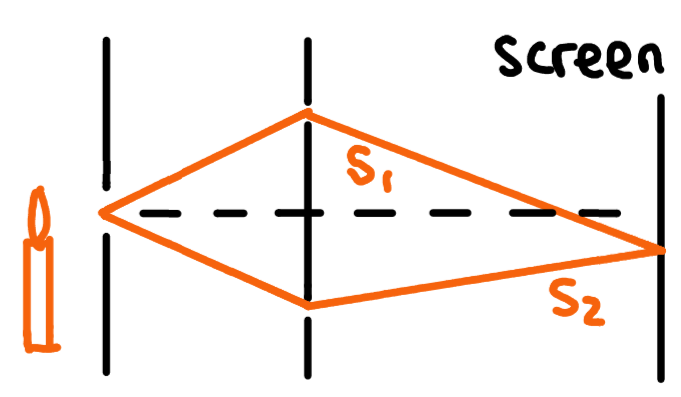
\includegraphics[width=\textwidth]{double_slit_1s}
    \newline
    在屏幕上,图案看起来像是这样
    \newline
    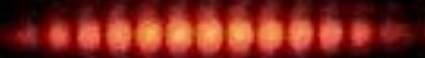
\includegraphics[width=\textwidth]{double_slit_2}
    \newline
    可以通过比较图中的$s_1$和$s_2$距离来计算屏幕上明亮条纹和暗淡条纹的位置。
    % $$s_1 = \sqrt{L^2 + (d+\delta)^2} \simeq s \left ( 1 + \frac{\delta d}{s^2}  \right )$$
    % $$s_2 = \sqrt{L^2 + (d-\delta)^2} \simeq s \left ( 1 - \frac{\delta d}{s^2}  \right )$$
    % $$s_1 - s_2 \simeq \frac{2\delta d}{s}~. $$ 
    \mtitem{
        \item  如果$s_1-s_2 = 0, \lambda, 2\lambda, \ldots$,那么来自两个轨迹的光朝同一方向振荡(相长干涉),并在屏幕上留下明亮条纹
        \item 如果$s_1-s_2 = \lambda/2, 3\lambda/2, \ldots$,然后来自两个轨迹的光向不同方向振荡(相消干涉),并在屏幕上留下暗淡条纹。
    }
    \tcblower
    要进行双缝实验,光波必须同时通过两条缝。如果我们挡住一个狭缝,原来的黑点就会变亮。
}
\textbox{光是粒子还是波:一个历史上的争论}{
    \titem{
        \item 早在公元前 400 年,德谟克利特\footnote{英语:Democritus,希腊语:Δημόκριτο(前460年—前370年或前356年),古希腊自然派哲学家。——译者注。}就断言万物都是由原子(微小粒子)构成的,包括光。
        \item In the early 17th century, optics was developing very fast led by microscopes, telescopes and so on. In 1630s, Descartes considered light as wave. In 1660, Grimaldi discovered diffraction of light, which behaves like water wave. 
        \item Newton discovered the dispersion of light (1666). He considered light as particles and dispersion is interpreted as mixing and separation of different particles (1672).
        \item Hooke and company strongly criticized Newton's particle theory of light and supported the wave theory.
        \item In 1704, Newton published ``Opticks'' (Hooke died in 1703). Due to his impact at that time, the particle theory of light dominated.
        \item In 1801, Young made a double-slit experiment. After that and further developements (for example the Poisson spot) the wave theory become dominate again.
        \item In 1861, Maxwell published his equations of E\&M. Electric field, magenetic field and light is then unified in one theory, where light appeared in the form of wave solutions. 
    }
}

Maxwell's equations concludes the  debate about the \emph{classical} nature of light -- light is wave, and its mathematical equations are found from the first principle. However, the nature of light starts to look surprisingly different again once we step into the modern era.

The whole thing started at an ``ultraviolet catastrophe''\index{ultraviolet catastrophe}\index{black body radiation}. The observed radiation from black body does not agree with Boltzmann's theory of statistical physics for short wavelength light. In 1900, Planck suggested that light is emitted and absorbed in a quantized way to solve the problem. This is the first indication of the quantum world historically. Here we will not follow a historical order, but instead show you two more intuitive experiments made slightly later, where classical physics fails.

\subsection{The Photoelectric Effect}

\textbox{The photoelectric effect\index{photoelectric effect}}{
    Consider the experiment in the margin figure.\marginnote{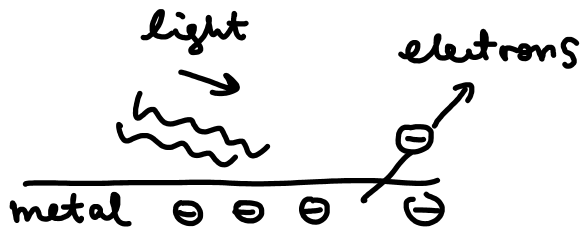
\includegraphics[width=0.3\textwidth]{photoelectric}} 
    A beam of light shines on metal. Apart of reflection light, what else do we expect to see?
    \titem{
        \item In 1887, Hertz noted that electrons can be knocked out by light. Such electrons are called photoelectrons. He also noted that the effect needs ultraviolet (UV) light.
        \item In 1902, Leonard studied the effect in more details. The energy of individual photoelectron increases with the frequency of light, but independent of the intensity of light. For each type of material, there is a cutoff frequency $\nu_0$, below which there is no photoelectron emission at all. The situation is plotted in the below figure.
    }
    \mtextbox{Summary of photoelectric effect}{
        \begin{tabular}{|c|c|c|} \hline
        Dependent on  & $I$   & $\nu$  \\ \hline
        \# of PE & Y   & N \\ \hline 
        Energy of PE & N & Y  \\ \hline
        threshold   & N & Y \\ \hline
        \end{tabular}
        \mnewline
        Here PE = photoelectron, $I$ and $\nu$ are the the intensity and frequency of the incident light, respectively.
    }
    \begin{center}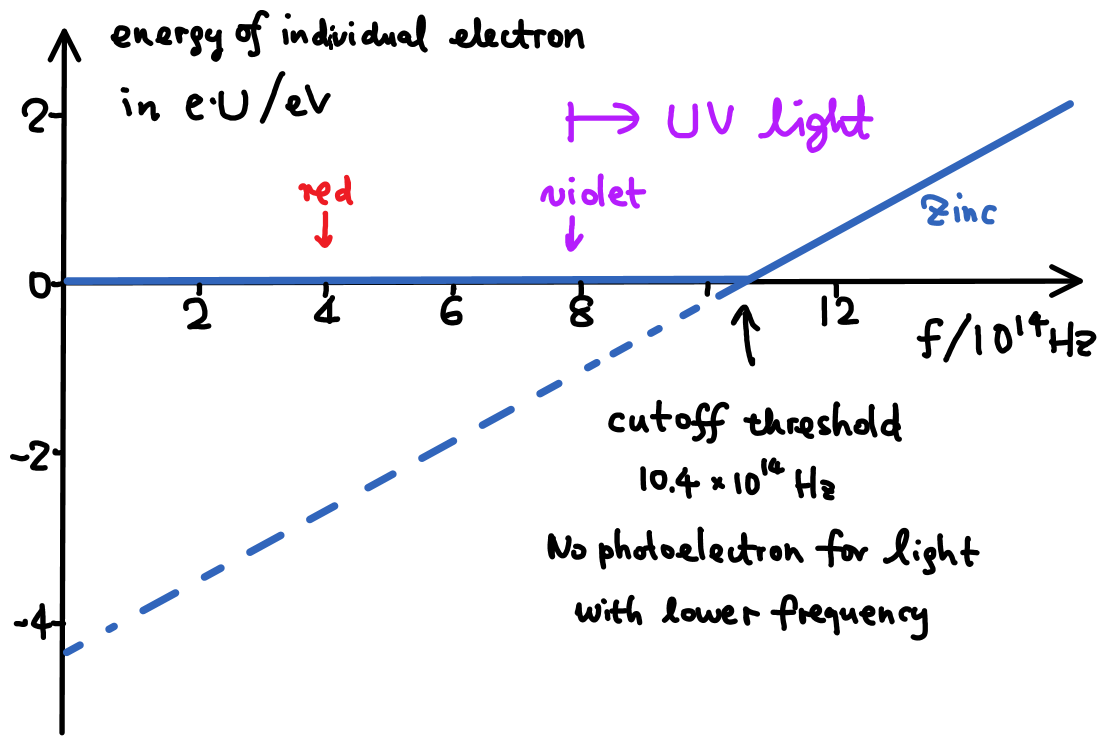
\includegraphics[width=0.7\textwidth]{photoelectric_plot}\end{center} 

    Why UV light with high enough frequency can knock out electrons? While light with lower frequency cannot knock out electrons no matter how strong is the beam of light. This surprising effect cannot be explained in classical E\&M, and gives us a clue about quantum mechanics.
}

Honestly, when I learned this I did not feel surprised though the textbook told me to feel so. Trust me, it's indeed surprising. If you are not convinced, let's instead think about the following game.

\textbox{The surprising whac-a-mole}{
    Whac-a-mole is a game to knock mice back to their holes. As physicists, instead of thinking how to knock them back, let's model why they come out. Assume they come out because they are scared by earthquake.

    \begin{center}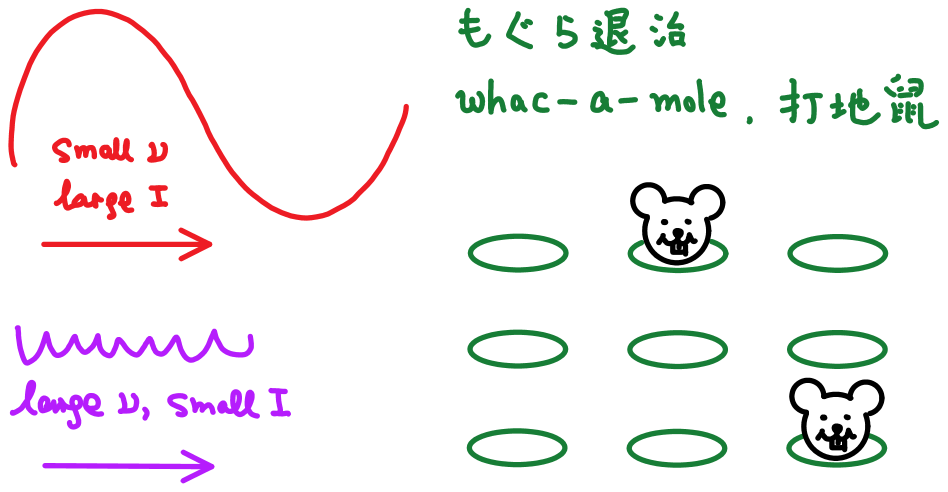
\includegraphics[width=0.7\textwidth]{whac}\end{center} 

    Imagine two types of earthquakes:
    \titem{
        \item Red earthquake has low frequency but very very large shaking amplitude.
        \item Violet earthquake has has high frequency but very very small shaking amplitude.
    }
    Which earthquake is more likely to scare mice out?
    \tcblower
    In reality, the red earthquake is of course more scary. But if we correspond this game to the photoelectric effect experiment, what the experiment tells is that
    \titem{
        \item The violet earthquake can scare some mice out despite of the small amplitude it has (indeed if it is stronger it can scare more mice out).
        \item No matter how strong the red earthquake is, it does no scare \emph{any} of the mice out.
    }
}

\mtextbox{Intensity still matters}{
    When photoelectrons can come out, the number of photoelectrons indeed depend on the intensity of light. The stronger light, the more photoelectrons. But the key puzzle is why the threshold of whether photoelectrons come out does not depend on intensity. 
}
\textbox{The photoelectric effect cannot be explained by classical E\&M}{
    Now have you started to feel that the photoelectric effect is surprising? Classical E\&M cannot explain photoelectric effect. In classical E\&M, electrons are shook by light, just as the mice shook by earthquake. When the intensity (i.e. shake amplitude) of the light is large enough, some electrons are shook so hard that they fly out of the metal. However, now whether electron leaves the metal depends on frequency instead of intensity. This poses a serious problem for the classical theory of light.
}

\mtextbox{Quantities describing waves}{
    \mtitem{
        \item Wavelength $\lambda$:\index{wavelength} length of a period of oscillation. 
        \item Wavenumber $k \equiv 2\pi /\lambda$:\index{wavenumber} number of radians the wave oscillates per unit distance. 
        \item Period $T\equiv \lambda/v$:\index{period} time duration of a period of oscillation. Here $v$ is the phase velocity of wave. For light, $v=c$.
        \item Frequency $\nu \equiv 1/T$:\index{frequency} number of oscillations per unit time. 
        \item Angular frequency $\omega\equiv 2\pi \nu$:\index{angular frequency} number of radians the wave oscillates per unit time.
    }
}
\textbox{Einstein's explanation of the photoelectric effect}{
    Inspired by Planck's 1900 explanation of black body radiation, Einstein proposed in 1905 that in the photoelectric effect, light can be considered as a collection of tiny particles (now known as \emph{photons}). Each photon has energy
    \begin{align}
        E = h \nu = h \frac{c}{\lambda} = \hbar \omega~,
    \end{align}
    where $h=6.6\times 10^{-34}\mbox{ m}^2\mbox{ kg s}^{-1}$ is the Planck constant, and $\hbar = h/(2\pi) = 1.1 \times 10^{-34}\mbox{ m}^2\mbox{ kg s}^{-1}$ is the reduced Planck constant. 
    
    This explains the photoelectric effect (and 王二's experience \ref{item:bullet} in her wonderland). Because an electron is likely to be hit by one photon instead of multiple photons together (if a person is hit by car, it is almost impossible that the person is hit by two cars at the same time). Thus whether the electron is knocked out of the metal is determined by the energy of the photon $E$, and thus its frequency $\nu$,  
    \mtextbox{Photon, quanta and quantization\index{photon}\index{quanta}\index{quantization}}{
        \mtitem{
            \item The ``tiny'' particle as building block of light is called photon.
            \item In general, the ``tiny'' particle (or quasi-particles where there is no actual particle) as building block of some form of energy (including matter itself, or the rotation, oscillation of matter, etc) is called quanta. In this sense, photon is the quanta of light. We will see that there are many other types of quantas that makes up our world.
            \item The feature that the quantas can be counted one by one (instead of being continuous) is that the quantas are ``quantized''.
        }
    }
    instead of the intensity of light. 

    Classical
    light can be considered a ``coherent state''\index{coherent state} of many photons. In a rough sense, coherent means that the $\mathbf{E}$ and $\mathbf{B}$ fields of the photons add coherently (instead of cancel each other in a disordered way).
}

\textbox{The everyday photoelectric effect}{
    We actually don't have to do experiments to find out the photoelectric effect. We know that strong sunlight hurts our skin. To reduce the hurt, we can use sunscreen (sun cream). For example, after applying SPF 30 sunscreen and stay under the sun for 30 minutes, in principle, your skin damage equals to staying 1 minute under the sun.

    How SPF 30 sunscreen works? To prevent damage to your skin (prevent sunlight reaching your skin), it should do either of the below for you:
    \titem{
        \item Reflection: reflect 29/30 of the light away. But, why you don't look like a mirror after applying sunscreen?
        \item Absorption: absorb 29/30 of the light before it reaches your skin. But, why don't you look black after applying sunscreen?
    }
    \tcblower
    This
    %\marginnote{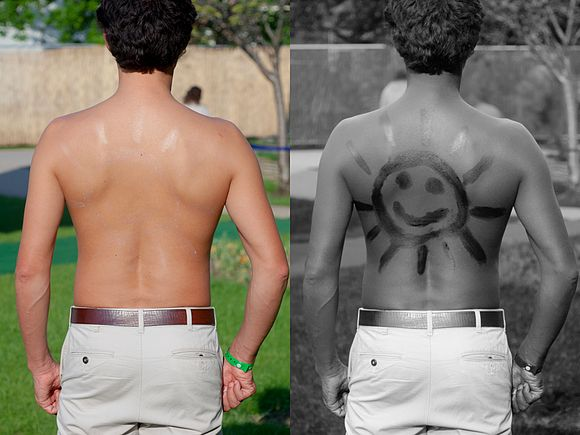
\includegraphics[width=0.35\textwidth]{Sunscreen_normal_UV} Photo after applying sunscreen. \newline Left: visible light; Right: UV light.}
    is because sunscreen does not reflect or absorb all frequencies of light. It is much more effective on UV light. Indeed you look different after applying sunscreen if you take a photo in the UV light frequency band.

    Why the UV light hurts your skin more than the visible light (which dominates energy of sunlight)? The reason is the same as the photoelectric effect (but what get knocked is not electrons but chemical bonds).

    \begin{center}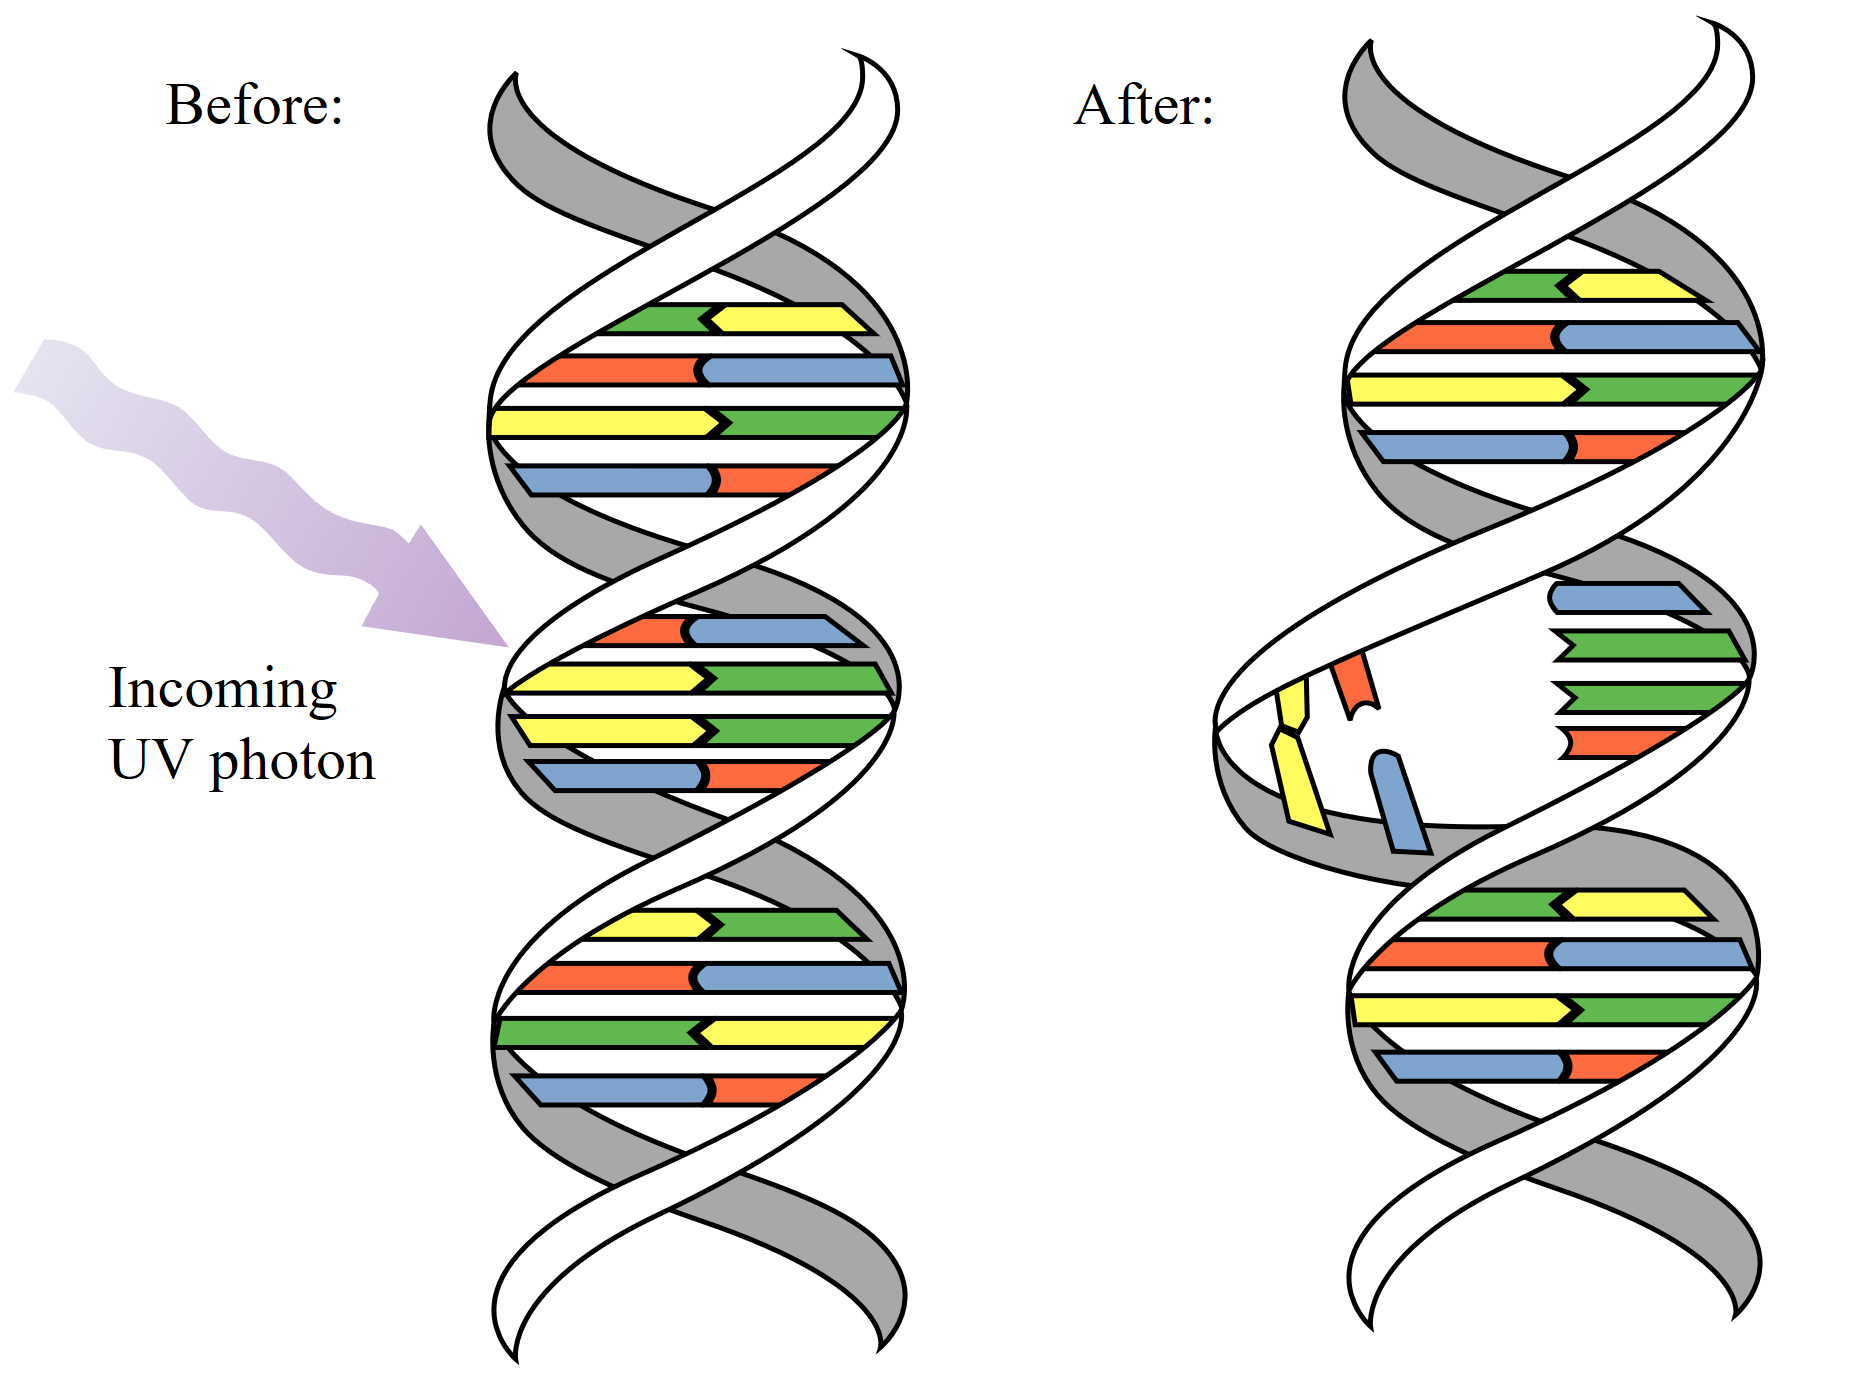
\includegraphics[width=0.4\textwidth]{dnauv}\end{center} 

    Also,\marginnote{And also you do not have to apply sunscreen when using your phone or microwave ovens, either.}
    in the winter, when you get close to a heater, you feel as warm as being under the sun. However, you don't have to apply sunscreen around a heater. This is because the heater radiation is dominated by the IR light. 
}

\textbox{Does the photon wavelength change? The Compton effect\index{Compton effect}}{
    In the photoelectric effect, we have discussed how the electrons behave when light shines on them. What about the photons themselves? Let the incoming photon wavelength be $\lambda$ and the outgoing photon wavelength be $\lambda'$. Are they equal?
    \marginnote{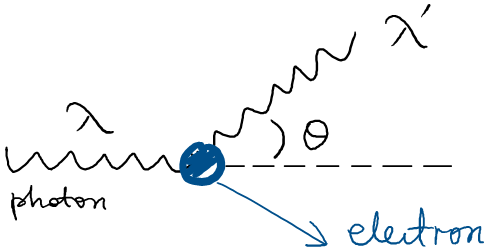
\includegraphics[width=0.3\textwidth]{compton}}
    \tcblower
    In classical E\&M, $\lambda = \lambda'$. The incoming light (which has oscillatory electric field) shakes the electrons, and then the shaken (i.e. accelerated) electrons runs away, at the same time emits outgoing light of the same frequency. 
    
    When the electrons got hit by light, they get additional kinetic energy. Where does the additional kinetic energy come from? In classical E\&M, the kinetic energy come from the reduction of the intensity of light, i.e. the outgoing light has small intensity. 

    However, the above energy argument must be wrong in a quantum theory. A photon cannot further reduce its intensity. Then, where would the kinetic energy of the electron come from? A photon has nothing to lose but its wavelength (recall $E=hc/\lambda$). Thus we must have $\lambda' > \lambda$. As a good exercise, assuming that the electrons are free without any binding energy, then energy-momentum conservation together with quantization $E=hc/\lambda $ gives
    \begin{align}\label{eq:compton}
        \lambda' - \lambda = \frac{h}{m_e c} \left ( 1-\cos\theta \right )~.
    \end{align} 
    Up to the angular factor $1-\cos\theta$, the shift of wavelength is $\lambda_c \equiv h/(m_e c) \simeq 2.4 \times 10^{-12}$m, known as the Compton wavelength. And the effect is observed by Compton (1923) and known as the Compton effect. Since the Compton wavelength corresponds to X-ray wavelength of light, the effect is hard to observe for observable light, and clearly visible when the wavelength of light is as short as X-ray.
}

\needspace{0.2\textwidth}
\mtextbox{Planck scale and quantum gravity}{
    In addition to the Bohr radius, we can also make another scale out of $\hbar$ once gravity is concerned. The scale is the Planck energy $E_p = \sqrt{\hbar c^5 / G} \sim 10^{9}\textrm{J} \sim 500$kWh, approximately the kinetic energy of an operating train. This scale puts together quantum and gravity, and is the scale of quantum gravity.
    \tcblower
    Consider two electrons, each has kinetic energy comparable to a running train, collide head-to-head. The collision is energetic enough to produce an microscopic black hole. Such collisions need to be studied with quantum gravity. We still don't have a full understanding of quantum gravity, though there is a decent candidate known as string theory.
}
\textbox{The dimension of $\hbar$}{
    It is interesting to note the dimension of $\hbar$: it connects mass, speed and length. This relates to the question: why there is a fixed size of atom, such that the electron does not fall into the nuclei. From dimension analysis, the electron mass is a fundamental quantity of nature. Through speed of light $c$ (enter from Coulomb's law) and $\hbar$ (and a dimensionless strength of interaction $\alpha$), the electron mass scale $m_e$ got converted to the atomic length scale $\hbar/(m_ec\alpha)$, known as the Bohr radius. Thus, from dimensional analysis, before putting in any dynamics, we already except that we need such a fundamental constant. We will see it explicitly in the part of atoms.
}

\textbox{Wait! Haven't you said that the particle theory of light is dead?}{
    In the last subsection \ref{sec:light-particle-wave}, I have already told you that the Newtonian particle theory of light is dead. Now, why Einstein dare to use particles to explain light again?
    \tcblower
    The photon that Einstein proposed is not a ``classical particle'' as we usually imagine. It has the feature of particles in that its energy is quantized and it appears to interact with the electron in the same way as two point particles collide. 

    Haven't I said that the particle theory of light contradict is killed by the double-slit experiment? Now let's see how the photons behave in the double-slit experiment.
}


\subsection{The Single Photon Double-Slit Experiment}

\textbox{The single photon double-slit experiment\index{double-slit experiment, single photon}}{
    In \marginnote{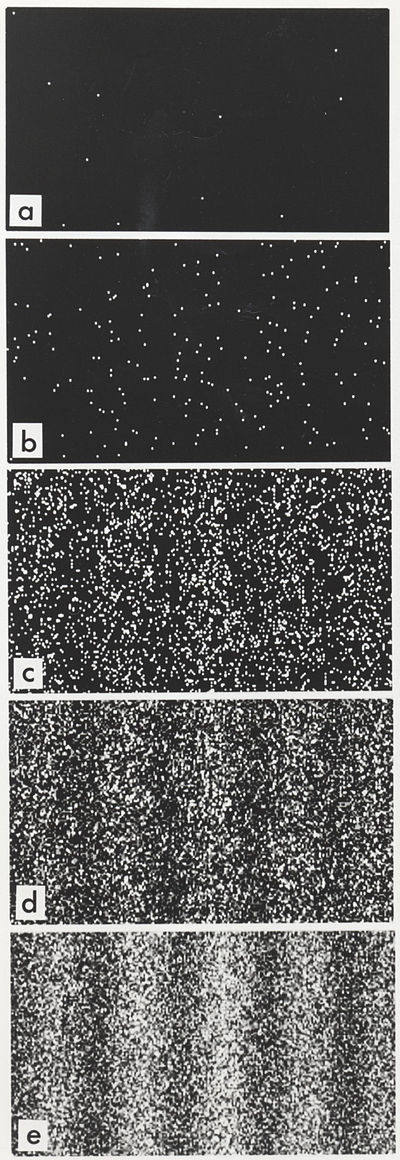
\includegraphics[width=0.35\textwidth]{double_slit_single_wikipedia}}
    section \ref{sec:light-particle-wave}, we have reviewed the double-slit experiment. Image that we reduce the intensity of light. Eventually, in the extremely-low intensity limit, each time we are doing double-slit experiment with only one photon. What is the outcome of such a single photon double-slit experiment? Suppose that we put a sensitive film on the screen which can record every photon. What's the status of the film as time goes on?

    The experiment was carried out in 1909 by Taylor. The result looks like the figures to the right. Two features are clearly spotted in the result:
    \tenum{
        \item At the early stage of the experiment (panels (a) and (b) of the figure), clearly, the photon postulate is supported: Indeed we see a few ``particles'' on the screen. Each photon leaves one point on the screen.
        \item As the experiment goes on (from panels (c) to (e)), more and more photons pass the slits. Interference patterns emerges. Indeed there are bright bands where the photons are more likely to reach and dark bands where the photons cannot reach.
    }
    \tcblower
    How to interpret this result? 
    
    Considering that the intensity of incoming light is low enough, one photon already reaches the screen and leaves an unchangeable record before the other photon starts off. Thus the photons can be considered as independent.
    
    Each photon behave independently but ends up at different points on the screen for the same experimental setup. Thus there must be some randomness in the photon behavior.

    So the position of a photon on the screen should satisfy a probability distribution (as a smoothed version of panel (e)). The probability is large at bright bands and vanishes at dark bands, forming interference patterns.
}

You may ask where the randomness come from. We will come back to this point when discussing quantum measurement. The short answer at the moment is that there is no unique fundamental answer to the origin of randomness. But we have a well-defined way to compute the probability distribution. In this section, let us focus on another question, along the line of particle-wave debate of light.

\needspace{0.2\textheight}
{}
\mtextbox{The which-way experiment\index{which-way experiment}}{
    You may want to further see which slit on earth the photon goes through. To do so, you put a detector on one of the slit. If the photon goes through this slit, the detector reports it. However, once a detector is placed, the interference pattern vanishes. 
    \tcblower
    There are many more confusing results, including compromise which-way experiment (1987), delayed choice (1999), weak measurement (2012), and so on. But here we have already enough surprises to explore at the moment and will not discuss these experiments here.
}
\textbox{Is a photon particle or wave?}{
    If you think the photon is a particle in the classical sense. Then recall how the interference patterns are formed:
    \titem{
        \item The photon must have gone through both slits. But how can a particle go through both slits at a time? Note that the photon is not supposed to further split into even smaller particles. Otherwise that contradicts the photoelectric effect, and contradicts the fact here that each photon leaves one point on the screen.
        \item The dark band of the interfernce pattern indicate destructive interference (cancellation between two branches). When particles meet, they collide. How can they stay at the same position and cancel each other?
    }
    \tcblower
    So you probably change your mind and consider photon as a wave in the classical sense. Then
    \titem{
        \item Why photons arrive at the screen one by one, and one photon is the smallest building block of energy? Can't we continuously reduce the energy of wave by continuously reduce the amplitude of oscillation?
        \item Why 
        \mtextbox{From double-slit to path integral}{
            (Optional) One can generalize the single-photon double-slit experiment by adding
            \mtitem{
                \item more slits on a board $A$
                \newline
                \begin{center}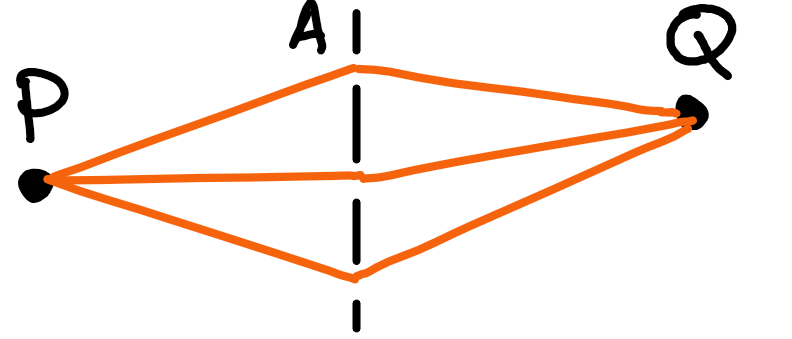
\includegraphics[width=0.6\textwidth]{dspi1}\end{center}
                \item more boards $A_1, A_2, \ldots, A_n$
                \newline
                \begin{center}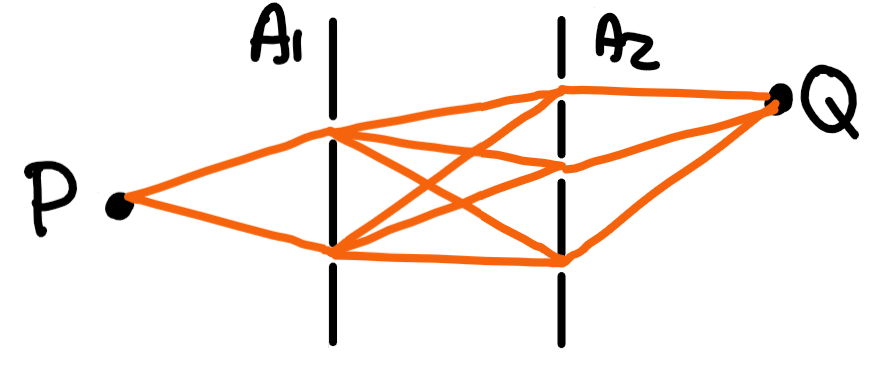
\includegraphics[width=0.65\textwidth]{dspi2}\end{center}
            }
            The interference pattern at $Q$ is the phase interference among all these paths. This should still apply if we have an infinite number of boards and each board has an infinite number of slits on it.
            \tcblower
            What does a board with an infinite number of slits mean? It can be considered as free space with no board at all! The probability amplitude of photon travelling in free space between $P$ and $Q$ can be computed by summing over the interferences of all paths. This approach is known as the path integral formulation of quantum mechanics, as mentioned in the part of action principle.
        }
        each photon leaves one point on the screen, instead of a weak but complete interference pattern?
    }
}

\subsection{A Wave-Particle Duality, and from Light to All Matter}

\textbox{A wave-particle duality\index{wave-particle duality}}{
    Is a photon particle or wave? This may be a wrong question to ask.

    We have listed the properties of particles and waves in section \ref{sec:light-particle-wave}. But who told us that microscopic matter must be classified into one of them following our classical experience?

    It turns out that microscopic matter has some natures of classical particles, and some natures of classical waves together. The full properties of classical particles or waves emerges exclusively in the classical limit when macroscopic matter is considered.
}

\textbox{Not only for photons, but for all matter quanta}{
    Now that light (considered waves before the quantum evolution) share some natures of particles, would matter like electrons, atoms, etc (considered particles before the quantum evolution) share some nature of waves as well?

    In 1924, de Broglie proposed that particle-like matter should also have wave-like properties. The de Broglie wavelength of a particle is proposed to be\index{matter wave}
    \begin{align}\label{eq:de-broglie-1}
        \lambda = h/p~.
    \end{align}
    Though sounds crazy at that time, the de Broglie matter wave is verified in experiments. For example, the interference patterns in the single photon double-slit experiment above is also observed using electrons, atoms, and so on. 
}

\needspace{0.2\textheight}
{}
\mtextbox{More success of matter wave}{In fact, crystal diffraction experiments are relatively easier ways to prove matter waves. The diffraction pattern of electrons are observed as early as 1927. Also the matter wave postulate immediately inspired Schr{\"o}dinger to ask the question: what is the wave equation of matter wave? He then derived the Schr{\"o}dinger equation in 1925 and published it in 1926.}
\textbox{Non-relativistic quantum mechanics}{
    Although quantum mechanics is initiated from photons, photons move at speed of light and thus is relativistic by its nature. The quantum theory consistent with special relativity (quantum field theory) was established much later than the non-relativistic quantum mechanics. This relativistic theory is beyond the scope of the current course. 

    Thus, now let us switch our attention from photons to massive microscopic particles, such as electrons, atoms, etc. They are non-relativistic at low energies. And our focus is how Newtonian mechanics get generalized into non-relativistic quantum mechanics. We will call non-relativistic quantum mechanics just quantum mechanics for short.
}

\mtextbox{(Optional) A field of particles}{
    The wave nature of particles provides us new insight about whether fundamental particles are the most ``fundamental'' objects. Think about water wave propagating on water surface. These water waves are not fundamental. They are excitations of the more fundamental water surface. Similarly, particles can be considered as excitations of more fundamental fields. For example, photons are excitations of E\&M field (which you have learned), and electrons are excitations of electron field (which you probably have not learned so far). The quantum theory of studying these more fundamental fields is known as ``quantum field theory'', which consistently put special relativity into the framework of a quantum theory.
    \tcblower
    In this course we restrict our attention to non-relativistic quantum mechanics. At this point it is fine to temporarily consider particles as ``fundamental'', and study their natures.
}
\textbox{The wave and particle properties of a quanta}{
    \titem{
        \item Quantized (particle-like). Quantas are discrete and can be counted.
        \item Superposition (wave-like). Like waves, quanta obeys linear equations of motion. One can thus add one solution and another to make a third solution. 
        \item Energy and angular frequency (connection of wave and particle). The particle-like energy and the wave-like angular frequency is related by the Planck formula
        \begin{align}
            E = \hbar \omega~.
        \end{align}
        \item Momentum and wavenumber (connection of wave and particle). The particle-like momentum and the wave-like wavenumber is related by the de Broglie formula \eqref{eq:de-broglie-1}
        \begin{align}
            p = \hbar k~.
        \end{align}
    }
    \tcblower
    We will expand some of these properties in great detail in the next section, and study a few other wave-like and particle-like properties in later sections.
}

\section{The Quantum Wave Function}

As we discussed, all matter has wave properties. How to describe wave? We are familiar with plane waves with angular frequency $\omega$ and wave number $k$, it looks like $\exp(i k x - i \omega t)$.\index{plane waves} It is a function of space and time, and a special example of wave function.

\mtextbox{What is the symbol $|\psi\rangle$?}{
    Don't be scared by the strange appearance of $|\psi\rangle$. For the moment being, it means nothing more than a state (the status of the quantum particle). In the part of quantum information, you will see why this notation is convenient. 
}
\textbox{The quantum wave function\index{wave function}}{
    We assert that a quantum state $|\psi\rangle$ is described by a wave function. For a quanta (quantum particle) moving in one spatial dimension, the wave function can be written as $\psi(x,t)$. In general, $\psi$ can take complex values. This wave function completely describes the quantum nature of the particle.
    \tcblower
    Why bother to introduce a wave function? What's its physical meaning? In the below subsections we will answer these questions. But before to proceed, let me remind you that at a given time, a whole function $\psi(x, t_0)$ contains much more information than the position and momentum of a particle (which are two real numbers). Thus a quantum state contains much more information than a classical state. We will see this again and again later.
}

\subsection{The Wave Function as a Probability Amplitude}

\textbox{The wave function is a probability amplitude}{
    From the single quanta double-slit experiment, we learned that we have to introduce probability into the theory of quantum mechanics in a fundamental way. 
    \marginnote{This explanation is first discovered by Born (1926).}
    The wave function is a probability amplitude, such that $|\psi(x,t)|^2$ is the probability density: 
    
    The \marginnote{For a complex number, $|\psi|^2 \equiv \psi^* \psi$, where star denotes complex conjugate.}
    probability to find the particle between $x$ and $x+dx$ is $|\psi(x,t)|^2 dx$.

    This is known as the Born's rule and is the physical meaning of the wave function.
}

\mtextbox{Why we want $\langle f(x) \rangle$?}{
    Because $\left\langle x \right\rangle$ does not provide us enough information about the distribution. We want to know more. For example, the two below distributions: 
    \newline
    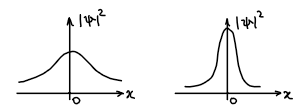
\includegraphics[width=\textwidth]{wave_function_moment}
    \newline
    They have the same $\left\langle x \right\rangle$. But in the left panel the value of $x$ is less certain because the distribution is broader, while in the right panel we have a better idea where to find the particle. This information is encoded in $\left\langle x^2 \right\rangle$.
}
\textbox{Features of the wave function in probability theory}{
    As a probability amplitude, we can immediately read off a few features of $\psi(x,t)$:
    \titem{
        \item The wave function is normalized as
        \begin{align}
            \int_{-\infty}^\infty |\psi(x,t)|^2 dx = 1~,
        \end{align}
        because it describes a particle, and the probability to find the particle once in the whole space is one.
        \item If we prepare many copies of the same state, and measure the position $x$ of the particle for each copy, the average value (called the \emph{expectation value}) of the position is
        \begin{align}
            \left\langle x \right\rangle = \int_{-\infty}^\infty x |\psi(x,t)|^2 dx~.
        \end{align}
        \item More generally, the expectation value\index{expectation value} for a function of position $f(x)$ is
        \begin{align}
            \label{eq:exp_fx}
            \left\langle f(x) \right\rangle  = \int_{-\infty}^\infty f(x) |\psi(x,t)|^2 dx
            = \int_{-\infty}^\infty \psi^*(x,t)~f(x)~\psi(x,t)~dx~.      
        \end{align}
    }
}

\textbox{Remaining questions}{
    We now already know a lot about the quantum state. However, you may have the following questions:
    \tenum{
        \item So far only $|\psi(x,t)|^2$ appears in the description. So why we use $\psi(x,t)$ as the fundamental object?
        \item How to relate $\psi(x,t)$ to the single quanta double-slit experiment?
        \item We have shown how to extract position information from $\psi(x,t)$. However, we need to extract the momentum information as well to know the state better. Can we and how do we do it?
        \item We have only discussed the $x$ dependence of $\psi(x,t)$, what about the $t$ dependence?
    }
    \tcblower
    We will address \enumlabel{1} and \enumlabel{2} in section \ref{sec:superposition}, \enumlabel{3} in section \ref{sec:wave-func-momentum}, and \enumlabel{4} in section \ref{sec:Schrod}.
}

\needspace{0.2\textheight}
\subsection{Consequence of Superposition and Linearity} \label{sec:superposition}

\mtextbox{Why probability amplitude?}{
    Now we know why we introduce probability amplitude in quantum mechanics: Because we treat probability as waves. Waves are linear in amplitude, but not in energy or intensity. This is a general feature of waves. For example, the intensity of light and the energy of water waves are both proportional to amplitude squared.
}
\textbox{The world is linear}{
    Superposition\index{superposition} is the key feature of wave. Mathematically, superposition means linearity: if wave functions $\psi_1$ and $\psi_2$ are solutions of the wave equation, then $c_1 \psi_1 + c_2 \psi_2$ is also a solution, where $c_1$ and $c_2$ are arbitrary complex-valued constants.
    
    The water waves and E\&M waves are approximately linear when the amplitude is small. However, quantum mechanics asserts that the wave function is \emph{exactly} linear.
}

\textbox{Double-slit and the interference in probability}{
    Suppose $\psi_1(x)$ and $\psi_2(x)$ are the solutions going through silt 1 and slit 2, respectively. Then from linearity, $\psi(x) = \psi_1(x) + \psi_2(x)$ is also a solution. From the symmetry of the double-slit setup, this should be the actual solution that we look for.\marginnote{Here we have written $\psi(x,t)\sim \psi(x)$ for a time-independent problem. We will later see that it is indeed consistent. Also, we are not careful about complex phases at this moment.}

    At the dark bands, though $\psi_1\neq 0$, $\psi_2\neq 0$, they cancel such that $\psi_1+\psi_2=0$.

    Thus, if we block a slit (say slit 2), the dark band is no longer dark since the probability density to have particle at the (originally) dark band is $|\psi_1|^2 \neq 0$. However, if we allow both slits, the probability density becomes $|\psi|^2 = |\psi_1+\psi_2|^2=0$.
    
    \mtextbox{Global and relative phases\index{global phase}\index{relative phase}}{
        \mtitem{
            \item Here, the relative phase (a phase is $e^{i\alpha}$ for real $\alpha$) between $\psi_1$ and $\psi_2$ has physical effects. Because the phase controls constructive interference, destructive interference or something in between.
            \item However, a global phase of the whole wave function $\psi$ (if we do not do further superpositions or enlarge the system) is unobservable (and thus unphysical). Because a global phase does not affect the probability density $|\psi|^2$.
        }
    }
    \tcblower
    Linearly adding up probability amplitude $\psi$ is how quantum mechanics. This is totally different from adding up probabilities in our classical life. 

    The probabilities are non-negative, and has no interference when adding them up. For example, if we buy a lottery and then buy another. The probability to win simply adds up. The probability of buying one lottery will not cancel the probability of buying the other.

    However, adding probability amplitude is different. Because
    \begin{align}
        |\psi|^2 = |\psi_1|^2 + |\psi_2|^2 + \psi_1^*\psi_2 + \psi_2^*\psi_1~.
    \end{align}
    The first two terms correspond to adding up probabilities. But there are two additional interference terms $\psi_1^*\psi_2 + \psi_2^*\psi_1$. They are not positive definite and can cancel the whole thing.
}
I hope this relates the single-quanta double-slit experiment to the wave function of a quanta, and explains 王二's observation \ref{item:double-door-interference} at the beginning of this part.

\textbox{Plane waves as building blocks of wave functions in free space}{
    In math, linearity allows us to expand the wave function with a complete set of basis. Physically, the importance of basis is that we can first understand these simple states, and then consider a general state as a weighted average of these simple states.

    The basis are the solutions of the wave equation and of course depend on detailed problems: for a particle moving in potential $V(x)$, the solutions (and thus basis) depend on the form of $V(x)$. For most of this part (unless explicitly stated), we will be interested in the case of a constant $V$ (or gluing a few stages of motion where each stage has constant $V$). For constant $V$, happily the basis of the wave function are the familiar plane waves
    \begin{align}
        \label{eq:plane_wave_psi}
        \psi_p(x,t) = \frac{1}{\sqrt{2\pi\hbar}}  e^{i(px-E t)/\hbar}~.
    \end{align}
    Here we have used $p=\hbar k$ and $E=\hbar \omega$ to replace wave vector and angular frequency with momentum and energy of the quanta. Positive and negative $p$ indicates that the wave is moving to the right and left, respectively. 
    \mtextbox{Plane waves are not normalized}{
    We required the $\psi$ being normalized: $\int  |\psi(x,t)|^2 dx = 1$. Unfortunately a plane wave cannot be normalized since this integral diverges for $\psi_k(x,t)$. Physically it is because finding the plane wave at anywhere in space is a constant: $|\psi_k(x,t)|^2=$ const. Thus the normalization factor (whose square is probability density) is zero. An analogue is that, if you guess an integer from 1 to 10, you can win by chance 1/10. But if you guess a number uniformly distributed from $-\infty$ to $\infty$, your chance to win is zero.
    \tcblower
    If you really worry about this normalization, you may choose to do one of the follows:
    %
    \mtitem{
        \item Start from finite volume of space, and take the volume of space infinity after all calculations.
        \item Consider a wave packet -- a collection of plane waves, which locally looks like plane waves but can be normalized properly. Physically, we can never make an exact plane wave 
    }
    But they make things unnecessarily complicated. We thus leave the plane waves unnormalized. The factor $1/\sqrt{2\pi \hbar}$ is not a normalization factor but just for future convenience.
    }
    %   
    Again, be reminded that by wave or oscillation here, there is nothing changing positions periodically as for water wave or E\&M wave. But rather what really oscillates is the \emph{probability amplitude}.
    \tcblower
    Thanks to linearity, a general state of quanta can be written as a superposition of the plane waves
    \begin{align}
        \label{eq:superposition_plane_wave_psi}
        \psi(x,t) = \int_{-\infty}^{\infty} dp ~ c(p) \psi_p(x,t)~,
    \end{align}
    where $c(p)$ are complex valued functions of $p$. Here $\psi(x,t)$ can be thought of as a weighted average of plane waves $\psi_p(x,t)$ with weight $c(p)$. And $c(p)$ can be thought of as how much of $\psi_p(x,t)$ is contained in a state $\psi(x,t)$.
}


Superposition opens up the possibility to consider more exotic objects, such as the Schr{\"o}dinger's cat (section \ref{sec:epilogue-qm}) and quantum entanglement (the next Part). 

\subsection{Extracting momentum information from the wave function} \label{sec:wave-func-momentum}

In Newtonian mechanics, to describe a state, we would like not only to know the position of the particles but also how they move (momentum). Now that a wave function describes the state of a quanta, we also would like to know how to extract the information of momentum from the wave function.

\textbox{States with certain and uncertain momentum}{
    What is the momentum of a wave function $\psi(x,t)$? We have a few observations:
    \titem{
        \item For plane wave $\psi_p$, we know that its momentum is $p$.
        \item For general $\psi$, we do not expect a definite answer because of superposition. For example, the state can be $\psi = \psi_{p_1} + \psi_{p_2}$ ($p_1\neq p_2$). What's the momentum of $\psi$? The state does not have a definite momentum, but rather we have probabilities to find the state with momentum $p_1$ and $p_2$.
    }
}

\mtextbox{Reconsidering normalizations}{
    You may be puzzled here: If I take $\psi = \psi_{p_1}$ and $\hat p = p_1$, then isn't $\int \psi_{p_1}^* p_1 \psi_{p_1} dx =\infty$?
    \mnewline
    You are right! This is because $\psi_{p_1}$ cannot be normalized.
    \mnewline
    To fix this, we may reconsider the expectation value and define:
    $\left\langle \hat p \right\rangle_r = \left\langle \hat p \right\rangle / \left\langle 1 \right\rangle$,
    \newline 
    where $\left\langle 1 \right\rangle \equiv \int \psi_{p_1}^* \psi_{p_1} dx$.
    \mnewline
    At first sight, this seems stupid: I am trying to make sense of $\infty/\infty$. However, in physics, this indeed makes sense: Plane waves in infinite space does not exist in its exact form in nature. This is the origin of the divergence. We thus can first \emph{regularize} the infinity by considering wave packets close enough to plane waves, or plane waves in a finite box. In such physical problems, the infinities are canceled and we get the desired result 
    $\left\langle \hat p \right\rangle_r = p_1$ for $\psi = \psi_{p_1}$.
}
\textbox{Computing expectation value involving momentum}{
    We have shown how to compute an expectation value $\left\langle f(x) \right\rangle$ for a function of position of the particle. For the momentum of the particle, we hope to find a similar formula
    \begin{align}
        \label{eq:exp_fp}
            \left<\hat p\right> = \int_{-\infty}^\infty \psi^*(x,t)~\hat p~\psi(x,t)~dx~.
    \end{align}
    Is it possible? Here we have put a hat to momentum $p$. Why? We hope $\hat p$ to tell information about momentum. However, we cannot simply take $\hat p = p$. Because the RHS does not have $p$ elsewhere in the equation. Thus putting a number $p$ in the integral does not make sense. So how to extract momentum information from the wave function?

    For example, if we take a plane wave $\psi=\psi_{p_1}$, we should expect $\hat p \psi_{p_1} = p_1 \psi_{p_1}$. If we take $\psi=\psi_{p_2}$, we should expect $\hat p \psi_{p_2} = p_2 \psi_{p_2}$. Is this possible for the same $\hat p$?

    This suggests that we take $\hat p$ as a differential operator (known as the momentum operator\index{momentum operator}), instead of a number:
    \begin{align}\label{eq:p-operator}
        \hat p = - i \hbar \frac{\partial}{\partial x} \equiv -i \hbar \partial_x~, 
    \end{align}
    where the $\partial_x$ in the very RHS is just a short hand notation of $\partial/\partial x$. We assert that \eqref{eq:p-operator} applies not only for free space, but also for non-constant $V$.
    \tcblower
    More generally, the expectation value $\left\langle f(x, \hat p) \right\rangle$ can be extracted from the wave function as
    \begin{align}
        \label{eq:exp_fxp}
            \left<f(x,\hat p)\right> = \int_{-\infty}^\infty \psi^*(x,t)~f(x,\hat p)~\psi(x,t)~dx~.
    \end{align}
}

\section{Observables and Measurements}

\marginnote{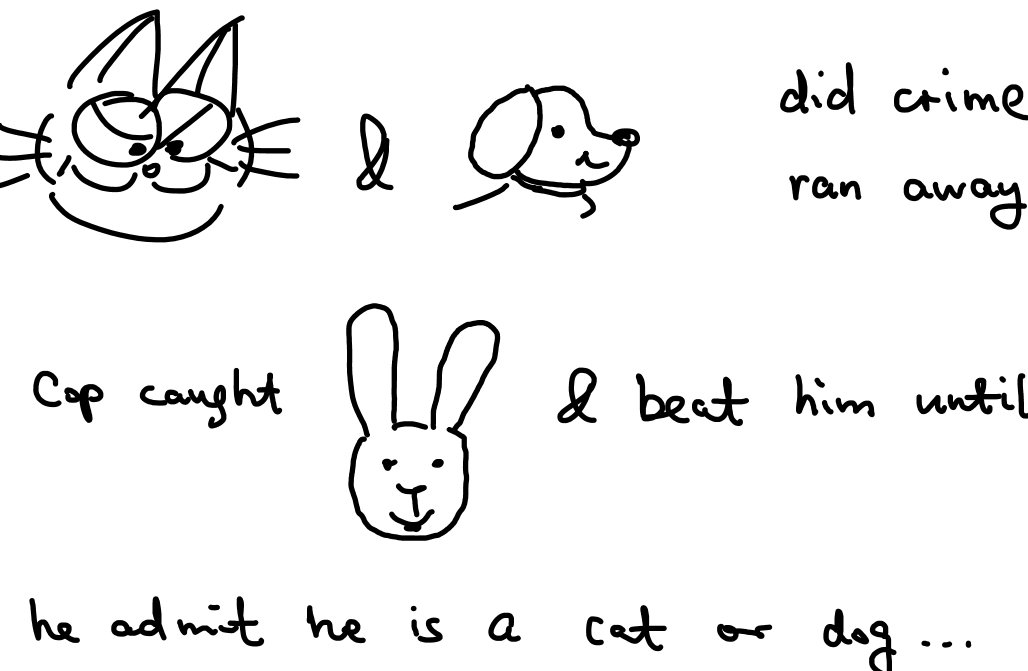
\includegraphics[width=0.35\textwidth]{measurements_cat_dog}}
When talking about expectation values in the previous section, we implicitly mean measurements: measuring many identical quantum states and take the average. In this section, let us address the question of measurements more carefully. Especially, if we only have one system and do a measurement once, how do we address the probability of measurement outcomes?

We have talked about a key difficulty: When measuring momentum, what happens if the state does not have definite momentum? In this section we will address the theory of measurements in quantum mechanics: observables, states and measurement outcome.

\mtextbox{Classical measurements are simple}{
    In classical theories, theorists never worried about measurements:
    \mtitem{
        \item A classical state always have definite values of observables.
        \item A classical measurement can be made in an infinitely gentle way which do not disturbe the system.
    }
    \tcblower
    Quantum systems do not have above features. Thus, measurement is a key part of the quantum mechanics theory.
}
\textbox{Observables are represented by operators\index{observable}}{
    To talk about measurements, we should start with what we can measure -- observables. For example, position and momentum are observables. In the example of momentum operator $\hat p = -i\hbar\partial_x$, we learned that a number may not be enough to represent an observable. For position, $x$ as a number can also be considered as a special operator $\hat x = x$. In general:

    An observable is represented by an operator $\hat O$ in quantum mechanics.

    Moreover, for the observable outcome being real numbers instead of complex numbers, we require that the observables are Hermitian operators: $\hat O^\dagger \equiv (\hat O^*)^T= \hat O$.
}

\textbox{States with definite values of observables\index{eigenstate}\index{eigenfunction}}{
    Among the quantum states, some states have definite value $\lambda$ of $\hat O$:
    \marginnote{In this section we will talk about the time around the measurement $t_m$ and suppress the time variable of the wave function for short: $\psi(x, t_m)\rightarrow \psi(x)$.}
    \begin{align}
        \hat O \psi_\lambda(x) = \lambda \psi_\lambda (x)~.
    \end{align}
    In other words, the operator acting on the wave function is equal to the number $\lambda$ acting on the state. For these states, when we measure $\hat O$ on the state, we get definite outcome $\lambda$. Mathematically, we call the state $\psi_\lambda(x)$ an eigenstate (or sometimes eigenfunction in math) of $\hat O$ with eigenvalue $\lambda$.

    \tcblower
    Examples:
    \titem{
        \item Momentum eigenstates: The plane waves are momentum eigenstates with definite momentum. Indeed, we already know that plane wave $\psi_{p}$ defined in \eqref{eq:plane_wave_psi}, and
        \begin{align}
            \hat p \psi_p(x) = p \psi_{p} (x)~.
        \end{align}
        When we measure the momentum of this state, we definitely get $p$.
        \item Position eigenstates: What kind of states have definite position? Recall the probability amplitude nature of the wave function, the state with definite position $q$ should only take value at one particular position $q$, and vanish everywhere else. This function is known as a Dirac $\delta$-function defined as\marginnote{Unfortunately, $\psi_q$ cannot be properly normalized either. Again, if you'd like to properly normalize $\psi_q$, you can either study particle in a finite box, or a physical narrow peak instead of the $\delta$-function.}
        \begin{align}
            \psi_q(x) = \delta(x-q) \equiv \begin{cases}
                0, & \text{if } x\neq q \\
                \infty \text{ with } \int_{-\infty}^{\infty} \delta(x-q)=1, & \text{if } x=q
              \end{cases}
        \end{align}
        We can test that $\psi_q(x)$ is indeed an eigenstate of $\hat x = x$:
        \begin{align}
            \hat x \psi_q(x) = q \psi_q(x)~. 
        \end{align}
        This is because if $x\neq q$, $\psi_q(x)=0$. We thus have $x \psi_q(x) = q \psi_q(x)$. When we measure the position of this state, we definitely get $q$.
    }
}

For the eigenstates, the outcome of measurement is simple: we get the corresponding eigenvalue once measured. However, what about superpositions, such as two plane waves $\psi_{p_1}+\psi_{p_2}$, or two Dirac $\delta$-functions $\psi_{q_1}+\psi_{q_2}$?

\mtextbox{``Collapse'' of wave function?\index{collapse of wave function}}{
    What does ``collapse'' of a wave function after a measurement mean? We mean the wave function becomes the corresponding eigenstate as indicated by the meaning of the word collapse. However, currently there is no unique understanding about dynamically why and how the collapse happen. This question is related to the interpretation of quantum mechanics. We will address it briefly in the epilogue section.
    \tcblower
    At the beginning of this part, when 王二 is walking in the brightness, her position keeps being measured. Thus she knows better where she is. This explains \ref{item:measure}.
}
\textbox{Measurement outcome for a general state}{
    For superpositions when measuring $\hat O$, we decompose the general state in eigenstates.
    \titem{
        \item For observables taking discrete results: The decomposition is
        \begin{align}
            \psi(x) = \sum_i c_i \psi_{\lambda_i}(x)~,
        \end{align}
        where $\psi_{\lambda_i}$ is the eigenstate of $\hat O$ with eigenvalue $\lambda_i$. The probability for the measurement outcome being $\lambda_i$ is $|c_i|^2$. After the measurement, the wave function ``collapse'' to $\psi_{\lambda_i}$.
        \item For observables taking continuous results: The decomposition is
        \begin{align}\label{eq:dec-lambda-continuous}
            \psi(x) = \int c(\lambda) \psi_\lambda ~ d\lambda~,
        \end{align}
        where $\psi_{\lambda}$ is the eigenstate of $\hat O$ with eigenvalue $\lambda$. The probability density for the measurement outcome being $\lambda$ is $|c(\lambda)|^2$. After the measurement, the wave function ``collapse'' to $\psi_{\lambda}$.
    }
    \tcblower
    Examples:
    \mtextbox{Wave Function Collapse Algorithm}{
        Interestingly, the collapse of the quantum wave function has inspired the classical programming world. The \href{https://github.com/mxgmn/WaveFunctionCollapse}{Wave Function Collapse Algorithm} is developed to dynamically generate infinitely sized 2D or \href{https://github.com/marian42/wavefunctioncollapse}{3D} maps. The algorithm is inspired by the quantum superposition and collapse of the wave function.
    }
    \titem{
        \item Momentum measurement: Equation \eqref{eq:superposition_plane_wave_psi} realizes equation \eqref{eq:dec-lambda-continuous}. After the measurement, the probability density to find $p$ is $|c(p)|^2$.
        \item Position measurement: A state $\psi(x)$ can always be written as
        \begin{align}
            \psi(x) = \int_{-\infty}^\infty \psi(q) \delta(x-q) ~dq~.
        \end{align}
        After the measurement, the probability density to find $q$ is $|\psi(q)|^2$. This reproduces the Born's rule, i.e. the probability amplitude interpretation of a quantum wave function.
    }
}

\section{The Uncertainty Principle} \label{sec:uncertainty}

We have lots of uncertainties in our classical life due to lack of information. For example, before your exam score is released, your teacher tells you only the mean and standard derivation (uncertainty) of score distribution. What can you tell from this information? If the standard derivation is small, you are more certain about your score, but less certain about your ranking (as a small mistake may bring you from top to below mean). If the standard derivation is large, you have less idea about your score but can estimate better your ranking based on usual performance.

In the quantum world, even if we have complete knowledge of the state, we still have uncertainties. For example, what happens if you measure the position of a plane wave?

In this section, let us make this question better defined and more general.

\textbox{Uncertainty is quantified by standard derivations}{
    Talking about precision (or uncertainty), the corresponding quantity in statistics is the standard derivation. Given a state:
    \titem{
        \item Uncertainty of the state's position $\sigma_x$ is
        $
            \sigma_x \equiv \sqrt{\left \langle \left ( x- \left \langle x \right \rangle \right )^2\right \rangle}
            = \sqrt{\langle x^2 \rangle - \langle x \rangle^2} ~.
        $
        \item Uncertainty of the state's momentum $\sigma_p$ is
        $
            \sigma_p \equiv \sqrt{\left \langle \left ( \hat p - \left \langle \hat p \right \rangle \right )^2\right \rangle}
            = \sqrt{\langle \hat p ^2 \rangle - \langle \hat p \rangle^2} ~.
        $
    }
}
\textbox{The uncertainty principle\index{uncertainty principle}}{
    In math, a 
    \href{https://en.wikipedia.org/wiki/Uncertainty_principle\#Wave_mechanics_interpretation}{Kennard inequality}
    tells that for $\hat p=-i\hbar \partial_x$:
    \begin{align} \label{eq:uncertainty-xp}
        \sigma_x \sigma_p \geq \frac{\hbar}{2} ~.
    \end{align}
    This is the uncertainty principle, first discovered by Heisenberg in 1927.
}

We are trying to pack all the difficulties into math. \marginnote{And going through the math proof does not make me feel it being more intuitive. That's why I choose to hide the math here and leave it for a proper quantum mechanics course. You will find it more intuitive once you realize that $\psi(x)$ and $c(p)$ are Fourier transform to each other. For Fourier transformation in general, the original function and the image admits an uncertainty principle. But this is beyond the scope of this course.} As a result, though \eqref{eq:uncertainty-xp} is a logical consequence, we do not have an intuitive understanding about what happens. Instead of proving \eqref{eq:uncertainty-xp}, let us see some examples.

\textbox{Understanding the uncertainty principle from waves}{
    Let's see a few examples of wave functions:
    \titem{
        \item Plane waves: $\psi_p = \frac{1}{\sqrt{2\pi\hbar}} e^{ipx/\hbar}$, $\sigma_p=0$ and $\sigma_x=\infty$.
        \item Gaussian wave packet:
        \begin{align}
            \label{eq:guassian_x}
            \psi(x) = \frac{1}{\sqrt{\sigma_x \sqrt{2\pi}}} e^{- \frac{x^2}{4\sigma_x^2} }~. 
        \end{align}
        It's simple to check that $\sigma_x$ is indeed the standard derivation for $x$. To calculate $\sigma_p$, noting that $\left\langle \hat p \right\rangle = 0$ and $\left\langle \hat p^2 \right\rangle = \hbar^2/(4\sigma_x^2)$. Thus $\sigma_p = \hbar / (2\sigma_x)$. The Gaussian wave packet exactly saturates the uncertainty principle.

        As the wave packet does not have definite momentum, different momentum eigenstates in the superposition do not move equally fast. That indicates that the wave packet will spread over time. We will see that it's indeed the case in section \ref{sec:Schrod}.
    } 
}

\mtextbox{Wave vs particle viewpoints}{
    There is a subtle difference between understanding the uncertainty principle from waves and particles: From waves, we are talking about the intrinsic fuzzyness of quantum states. This is more precise in the sense of a princple of uncertainty. From particles, we see that fundamentally when measuring a microstate's position we have to change its momentum. These two aspects are nevertheless consistent with each other.
}
\textbox{Understanding the uncertainty principle from particles}{
    Can we first measure $x$ and then measure $\hat p$ for the same state, and thus get both position and momentum information precisely?

    The quick answer is no, because after a quantum measurement, the state collapses to the eigenstate. But this argument still seems mysterious. Let us consider a scenario in which we can see what actually happens.

    \tcblower

    Any measurement must act some interaction on the system and thus must change the system. 
    
    For example, you see an apple because light is reflected by the apple and is detected by your eyes. The light pushes the apple at the same time.

    Classically, the reaction on the system can be made as small as one wants. However, quantum mechanically it is not possible. 

    To measure the position precisely, one needs to use a wave packet of light with shorter wavelength. We at best have $\sigma_x \sim \lambda$.
    \marginnote{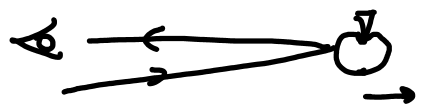
\includegraphics[width=0.35\textwidth]{light_on_apple}}

    From de Broglie's relation, $p_\lambda \geq \hbar/\lambda$ and thus shorter wavelength implies larger $p_\lambda$. The reflection of light transfers momentum of order $p_\lambda$ to the measured object. Thus the object has a momentum uncertainty of order $\sigma_p \sim p_\lambda$. As a result, we at least need $\sigma_x\sigma_p \sim \hbar$.
}

\mtextbox{What is possible about cloning}{
    It's important to note the conditions of the non-cloning theorem.
    \mtitem{
        \item It is possible to produce many copies of a known state. However, the ability of producing a known state does not help you to measure the position and momentum of an unknown state.
        \item It is possible to clone a state and at the same time destroy the original copy. Observiously this does not help you to invalidate the uncertainty principle either.
    }
}
\textbox{Optional: The quantum non-cloning theorem\index{quantum non-cloning theorem}}{
    You may think of another way to invalidate the uncertainty principle: What about clone the state into two copies, and measure position and momentum respectively?

    Unfortunately, your brilliant idea has been elaborately blocked by the theory of quantum mechanics, by the quantum non-cloning theorem -- no machine can clone an unknown state without destroying the original copy.

    \tcblower

    To prove that, we need to extend our language a little: including states of a cloning machine and multiple outcome states. Also, it is convenient to use the abstract notation $|\mbox{object}\rangle$ to denote the quantum state of the object. If a quantum cloning machine $|M\rangle$ exists, it does the follows: for any given quanta state $|\psi\rangle$, the machine transforms the state as
    \begin{align}
        |M\rangle |\psi\rangle \rightarrow |M_\psi \rangle |\psi\rangle |\psi\rangle ~,
    \end{align}
    where $|M_\psi\rangle$ is the state of the machine after the transformation. Now, consider two states $|1\rangle$ and $|2\rangle$. We expect 
    \begin{align}
        |M\rangle |1\rangle \rightarrow |M_1 \rangle |1\rangle |1\rangle ~,
        \qquad
        |M\rangle |2\rangle \rightarrow |M_2 \rangle |2\rangle |2\rangle ~.
    \end{align}
    Now what about the state $\alpha |1\rangle + \beta |2\rangle$?
    \tenum{
        \item From how a cloning machine should work, we should get $|M_*\rangle \left ( \alpha |1\rangle + \beta |2\rangle \right)^2$.\label{enum:clone1}
        \item From linearity of quantum mechanics, we should get $\alpha |M_1 \rangle |1\rangle |1\rangle + \beta |M_2 \rangle |2\rangle |2\rangle$.\label{enum:clone2}
    }
    Although we don't know the final state of the machine $|M_1\rangle$, $|M_2\rangle$ and $|M_*\rangle$, the above \ref{enum:clone1} and \ref{enum:clone2} cannot be consistent. Because \ref{enum:clone1} contains $\alpha\beta|1\rangle|2\rangle$ which is not part of \ref{enum:clone2}. We thus conclude that a quantum cloning machine is impossible. Linearity is the key to prove the non-cloning theorem.
}

A joke says when Heisenberg knows where he is, he doesn't know how fast he is walking. So does 王二 for item \ref{item:uncertainty} at the beginning of this part.


\section{The Schr{\"o}dinger Equation} \label{sec:schro-all}
We have talked about the interpretation of quantum states and measurements. They belong to the properties of the state at a given time.

But more importantly, physics is about given an initial condition, how to predict the state after some time. In other words, it is important to know the equation of motion which governs the time evolution of the system. In quantum mechanics, this governing equation is the Schr{\"o}dinger equation.

\needspace{0.2\textheight}
\subsection{The Schr{\"o}dinger Equation} \label{sec:Schrod}

\mtextbox{We are not deriving it}{
    Here by arguments and extrapolations, we show that the Schr{\"o}dinger equation is a natural thing to expect. But we are not deriving the Schr{\"o}dinger equation. Rather, the Schr{\"o}dinger equation is a fundamental postulate of quantum mechanics.
    \tcblower
    The Schr{\"o}dinger equation appears to be derived here because we have treated: The plane waves are the quantum state in free space with $V=$ const (even for constant $V$, we only argued that the plane waves are the natural thing to expect). But now, we are extrapolating to include non-constant $V$.
}
\textbox{Extracting energy from a wave function: the Schr{\"o}dinger equation\index{Schr{\"o}dinger equation}}{
    We discussed in section \ref{sec:wave-func-momentum} that the operator $-i\hbar \partial_x$ can extract momentum from a plane wave $\psi_p(x,t)\propto \exp[i(p x - E t)/\hbar]$, and consequently any superposition of plane waves, and thus a general wave function.

    How to extract the information of energy from a wave function? We can do it in two ways:
    \tenum{
        \item Using the relation $E = \frac{p^2}{2m} + V(x)$
        and replacing $p\rightarrow \hat p$.
        \item Noting that applying $i\hbar \partial_t$ on plane waves directly extract their energies.
    }
    These two ways must be consistent. We thus get an equation
    \begin{align}
        \label{eq:Sch-eq}
        i\hbar\partial_t \psi(x, t) = \hat H \psi(x, t)~,
        \qquad \hat H \equiv -\frac{\hbar^2\partial_x^2}{2m} + V(x)
    \end{align}
    This is the Schr{\"o}dinger equation, and $\hat H$ is called the Hamiltonian (the operator corresponding to energy). The LHS connects the state of a given time to a later time by the appearance of $\partial_t$.
    \tcblower
    In this part, we have been talking about one-dimensional problems. For future reference, the Schr{\"o}dinger equation with three spatial dimensions takes the form
    \begin{align}
        \label{eq:Sch-eq-3d}
        i\hbar\partial_t \psi(\mathbf{x}, t) = \hat H \psi(\mathbf{x}, t)~,
        \qquad \hat H \equiv  -\frac{\hbar^2\nabla^2}{2m} + V(\mathbf{x})
    \end{align}      
}

\mtextbox{Why spreading?}{
    Why the wave packet is spreading? Intuitively, a wave packet contains waves with different momentum. These waves travel at different speeds. Thus, after a while, the superposition disperse and the wave packet spreads.
}
\textbox{The spreading wave packet\index{Gaussian wave packet}}{
    We have argued that wave packets spread because its uncertain momentum. How to see this in calculations?

    Let us focus on the simplest case: $V=0$. One can verify that the following wave function satisfies the Schr{\"o}dinger equation:
    \begin{align}
    \label{eq:gaussian_psi}
    \psi(x,t) = \sqrt{\frac{\sigma}{\sqrt{2\pi}(\sigma^2+i\beta t)}}
    e^{i(kx-\omega t)} e^{- \frac{(x-v_gt)^2}{4(\sigma^2+i\beta t)} }
    \end{align}

    where $v_g \equiv \hbar k/m$, $\beta \equiv \hbar/(2m)$ and $\omega \equiv \hbar k^2/(2m)$. Here $\sigma$ is a free parameter, indicating the spatial spread of the wave function at $t=0$. 

    This solution is known as the Gaussian wave packet because the probability density is
    \begin{align}
    \label{eq:gaussian_prob}
    |\psi(x,t)|^2 = \frac{\sigma}{\sqrt{(2\pi)(\sigma^4+\beta^2 t^2)}}
    e^{- \frac{\sigma^2 (x-v_g t)^2}{2(\sigma^4+\beta^2 t^2)} }~. 
    \end{align}
    This is indeed a Gaussian wave packet at any time. The spatial spread of the wave function is
    \begin{align}
    \label{eq:gaussian_sigma_x_t}
    \sigma_x(t) = \sqrt{\sigma^2 + \frac{\beta^2t^2}{\sigma^2}}~.
    \end{align}
}

\textbox{The stationary state Schr{\"o}dinger equation\index{stationary state Schr{\"o}dinger equation}}{
    Solutions of the Schr{\"o}dinger equation with definite energy $E$ is of particular interest. This is because:
    \titem{
        \item Physically, energy is conserved. If we start with a state with definite energy and keep it isolated, it will continue to have definite energy. 
        \item Mathematically, with definite energy, the Schr{\"o}dinger equation is greatly simplified. In general, the Schr{\"o}dinger equation \eqref{eq:Sch-eq} is a partial differential equation. For a state with definite energy, we can solve the time part trivially and reduce it to an ordinary differential equation in the $x$ direction only.
    } 
    \tcblower
    For a state with definite $E$, the Schr{\"o}dinger equation breaks into two parts:
    \titem{
        \item The time part is $i\hbar\partial_t \psi(x,t)= E \psi(x,t)$. This can be solved as $\psi(x,t) = e^{-i E t/\hbar} \psi(x)$. Thus the time dependence in the wave function is a simple phase.
        \item The Hamiltonian part is
        \begin{align}
            \label{eq:Sch-eq-static}
            \left[ 
                -\frac{\hbar^2\partial_x^2}{2m} + V(x) 
            \right] \psi(x) = E \psi(x)~.
        \end{align}
        This equation is known as the stationary state Schr{\"o}dinger equation.
    }
}

The stationary state Schr{\"o}dinger equation \eqref{eq:Sch-eq-static} is a powerful tool to explore the quantum wonderland. In the reminder of the section, we will make use of the stationary state Schr{\"o}dinger equation to consider various types of potentials and how the wave function $\psi(x)$ behaves in these cases.

\subsection{A Step in the Potential}

Here and in subsequent subsections, we focus on square potentials where the potential is a constant at most places, except having a sudden change at the connection points. For such potentials, plane waves still work at almost everywhere, except that at connection points continuous conditions have to be imposed. This avoids the math difficulty of solving the Schr{\"o}dinger equation as a differential equation.

\mtextbox{Realization of a step}{
    For example, a charged quanta travelling from zero electric potential to non-zero electric potential realizes a step potential if the transition is sharp.
    \newline
    \begin{center}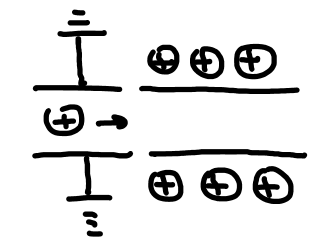
\includegraphics[width=0.6\textwidth]{step_potential}\end{center}
}
\twocol{0.55}{0.05}{0.37}{
    \textbox{The step potential\index{potential: step}}{    
    Consider the potential in the stationary state Schr{\"o}dinger equation \eqref{eq:Sch-eq-static}:
        \begin{align}
            \label{eq:step_potential}
            V = 
            \begin{cases}
              V_1, & \text{if } x<x_0 \\
              V_2, & \text{if } x>x_0
            \end{cases}
        \end{align}}
}{
        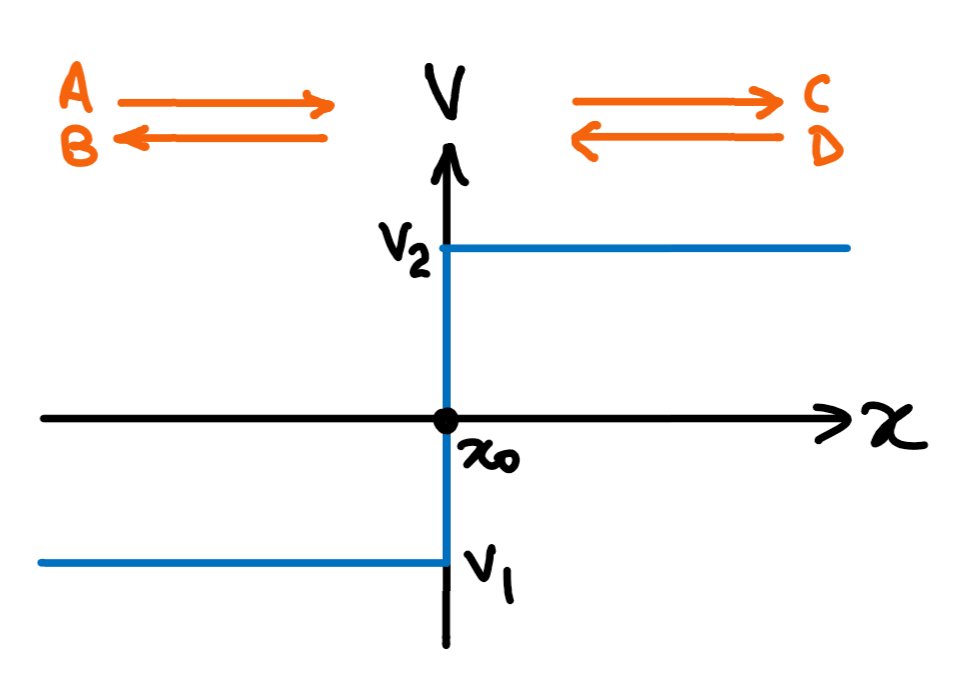
\includegraphics[width=\textwidth]{step_potential_1}
}

Labels $A$, $B$, $C$, $D$ in the figure will be used in the box below.

\textbox{Wave function away from the step}{
    For the step potential, when $x\neq x_0$, $V$ is a constant. The stationary state Schr{\"o}dinger equation reduces to
    \begin{align}
    \label{eq:sch_step_ABCD}
    - \frac{\hbar^2}{2m} \partial_x^2 \psi(x) = (E-V) \psi~.
    \end{align}
    It has very simple solutions. It is the same plane wave solutions which have motivated us to ``derive'' the Schr{\"o}dinger equation:
    \begin{align}
    \label{eq:sol_step_ABCD}
    \psi(x) =
    \begin{cases}
        A e^{ik_1 x} + B e^{-ik_1 x}, & \text{if } x<x_0 \\
        C e^{ik_2 x} + D e^{-ik_2 x}, & \text{if } x>x_0
    \end{cases}
    \end{align}
    where $A$, $C$ denote waves moving to the right, $B$, $D$ denote waves moving to the left, and 
    \begin{align}
    \label{eq:sol_step_ABCD_k12}
    k_1 \equiv \frac{1}{\hbar}\sqrt{2m(E-V_1)}~,
    \quad
    k_2 \equiv \frac{1}{\hbar}\sqrt{2m(E-V_2)}~.
    \end{align}
}

\textbox{The connection conditions\index{connection conditions of wave function}}{
    What happens to the point $x_0$? There must be two relations between $A$, $B$, $C$ and $D$. This is because, mathematically, Eq. \eqref{eq:sol_step_ABCD} is a second order differential equation and thus should have only two integration constants. Physically, if we set $D=0$, then it becomes a problem of an incoming wave $A$ scatter at the potential and thus $B$ and $C$ should be fixed. Thus there are two relations between $A$, $B$, $C$ and $D$.

    The relations are
    \titem{
        \item $\psi(x)$ is continuous. Otherwise, $\partial_x \psi(x_0)\rightarrow\infty$ $\Rightarrow$ infinite momentum $\Rightarrow$ unphysical.
        \item $\psi'(x)$ is continuous. Otherwise, $\partial_x^2 \psi(x_0)\rightarrow\infty$ $\Rightarrow$ infinite energy $\Rightarrow$ unphysical.
    }
    Applying these two relations to connect the two branch of solutions in Eq. \eqref{eq:sol_step_ABCD}:
    \begin{align}
    \label{eq:rel_step_ABCD}
    A e^{ik_1x_0}
    =& \frac{k_1+k_2}{2k_1} C e^{i k_2 x_0}
    + \frac{k_1-k_2}{2k_1} D e^{-ik_2 x_0}~,
    \nonumber\\
    B e^{-ik_1x_0}
    =& \frac{k_1-k_2}{2k_1} C e^{i k_2 x_0}
    + \frac{k_1+k_2}{2k_1} D e^{-ik_2 x_0}~,  
    \end{align}
}

\textbox{Scattering into classically allowed region with $E>V_1$ and $E>V_2$\index{classically allowed region}}{
    As we mentioned, when setting $D=0$, the problem is reduced to a scattering problem. $A$ is the incoming wave coming from $x\rightarrow -\infty$, $B$ is the reflection wave and $C$ is the outgoing transmission wave. 

    Here we first consider the case when the energy of the state is large enough, such that if the state was a classical particle, then it is able to reach $x>x_c$ regime.

    From Eq. \eqref{eq:rel_step_ABCD} we get
    \begin{align}
    \label{eq:rel_step_ABC}
    C & = \frac{2k_1}{k_1+k_2} e^{i(k_1-k_2)x_0}A~,
    \nonumber\\
    B & = \frac{k_1-k_2}{2k_1} e^{i(k_1+k_2)x_0}C
        = \frac{k_1-k_2}{k_1+k_2} e^{2ik_1x_0} A~.
    \end{align}
    In general, there are transmission and scattering waves. This is different from the particle mechanics that the particle always goes through (because it has enough energy).
}

\textbox{Scattering into classically forbidden region with $V_1<E<V_2$\index{classically forbidden region}}{
    Now we consider the case $E<V_2$. In this case, classically the particle is unable to reach the $x>x_c$ regime.

    In this case, $k_2$ becomes imaginary. When $x>x_0$,
    \begin{align}
    \label{eq:step_xgx0}
    \psi(x) = C e^{-|k_2|x}~.
    \end{align}
    We are forced to have $D=0$ because the $D$ term blows up at $x\rightarrow\infty$. The formal solution of $C$ is the same as Eq. \eqref{eq:rel_step_ABC}.

    \marginnote{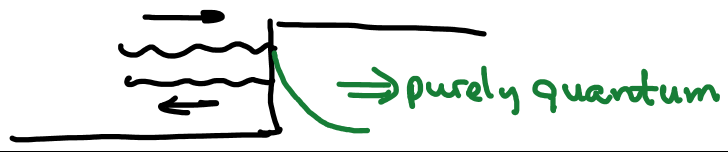
\includegraphics[width=0.3\textwidth, trim={0 3pt 3pt 0}, clip]{classical_forbidden}}
    How the particle can enter the classical forbidden regime even if the $V_2>E$? This is because formally the effective ``kinetic energy'' $\hbar^2 k_2^2 /(2m)<0$ when $k_2$ is imaginary.

    \marginnote{However, in the wave perspective, it is not that hard to understand -- E\&M wave into a conductor has similar exponentially decaying properties (instead of vanish immediately).}
    An exponentially small part of wave function can enter the classical forbidden regime. This is completely different from classical particles and has profound implications. We shall uncover some of them later, namely tunneling, a consistent picture of identical particles.
}

\subsection{The Potential Barrier: Reflection and Tunneling}

Now we modify the step potential further: Let's join two steps to make a potential barrier.

\textbox{Scattering on a potential barrier\index{potential: barrier}}{
    Consider \marginnote{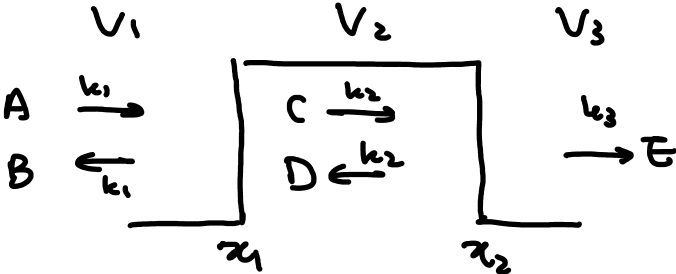
\includegraphics[width=0.35\textwidth]{potential_barrier}}
    the potential barrier illustrated in the figure. The detailed calculation will be left as an exercise. And here we shall use the experience we got from the step potential to study qualitative features here.

    The way of solving this problem is similar to the last subsection: In principle we just have to solve an array of 4 equations at $x_1$ and $x_2$, to determine 4 relations between 5 coefficients. 

    Practically, it is convenient to start from the outgoing wave $E$. Given $E$, we get $C$ and $D$. And given $C$ and $D$, we get $A$ and $B$. In other words, given non-vanishing $A$, we always have non-vanishing $E$, even in the case that $E<V_2$.
}

\needspace{0.1\textheight}
\marginnote{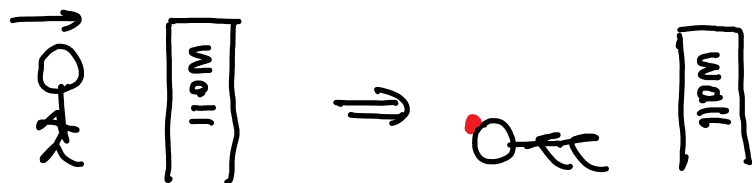
\includegraphics[width=0.35\textwidth]{tunneling_classical}}
\textbox{The quantum tunneling effect\index{tunneling}}{
    In the case $E<V_2$, classically the particle can never go from $A$ to $E$ because there is a barrier to block it. 

    However, \marginnote{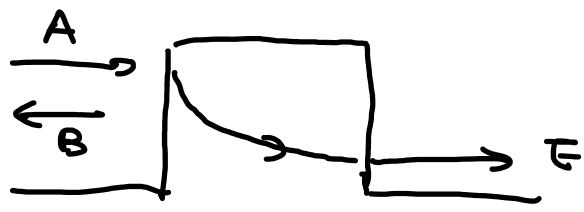
\includegraphics[width=0.35\textwidth]{tunneling_quantum}\newline This is why at the beginning of this part, the quantum 王二 observe that she can sometimes walk into a wall to enter a room in item \ref{item:cross-wall}.}
    in quantum mechanics, no matter how high the barrier is (in the real world the barrier is always finite), there is an exponentially small part which goes into the barrier and escapes out to $E$. This is a key feature of quantum mechanics.
}

\textbox{Example of tunneling: $\alpha$-decay\index{$\alpha$-decay}}{
    Heavy elements may be unstable. They may emit an $\alpha$ particle, i.e. the Helium nuclei ${}_2^4He$ and the remaining part becomes another element. This process is known as the $\alpha$-decay. 

    \marginnote{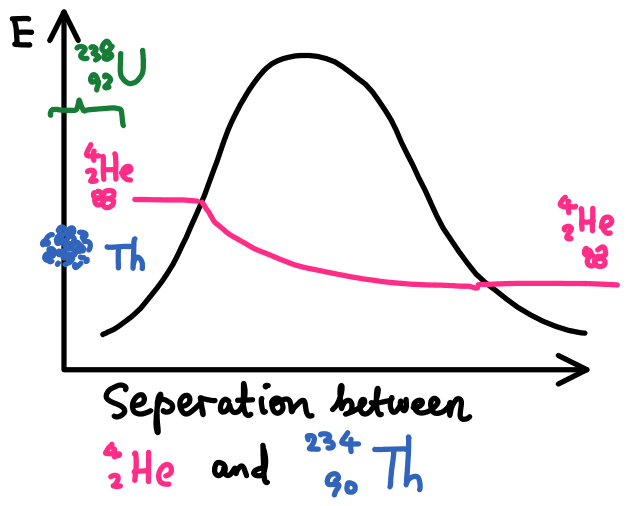
\includegraphics[width=0.35\textwidth]{qm_alpha_decay}} 
    For example, the following process can happen:
    \begin{align}
    \label{eq:alpha_example}
    {}_{92}^{238}\mathrm{U} \rightarrow 
    {}_{90}^{234}\mathrm{Th} + {}_2^{4}\mathrm{He}~.
    \end{align}
    Here the ${}_{90}^{234}\mathrm{Th}$ part of the nuclei provides a binding potential for the ${}_2^{4}\mathrm{He}$ part of the nuclei. They are together to form the ${}_{92}^{238}\mathrm{U}$. But the ${}_2^{4}\mathrm{He}$ has a small chance to escape, and this is the $\alpha$-decay of ${}_{92}^{238}\mathrm{U}$.

    The element ${}_{92}^{238}\mathrm{U}$ has a half-life of $10^{17}$ seconds $\sim 4\times 10^9$ years (about 1/3 of the age of the universe). Note that the time scale of a typically microscopic process
    is often a tiny fraction of a second. Such a huge difference in time scales is because of the exponentially small decay rate. 
}

\subsection{The Potential Well: Scattering and Bound States}

What about to connect the two steps differently, to form a potential well?

\textbox{The potential well\index{potential: well}}{
    Consider \marginnote{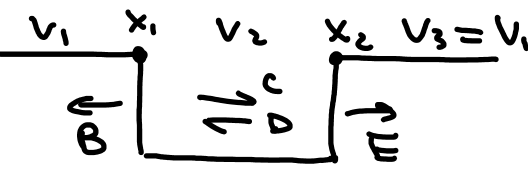
\includegraphics[width=0.35\textwidth]{potential_well}} 
    a potential well as in the side figure. The energy of the quanta classifies the problems into two cases:
    \titem{
        \item High energy scattering problem: If $E>V_1$ and $E>V_3$, the situation is similar to the discussion in the last subsection.
        \item Low energy bound state: What if $E<V_1$ and $E<V_3$? There is no wave coming from $x\rightarrow -\infty$ or wave going towards $x\rightarrow\infty$. As a result, the quantum state is confined inside (or a little bit outside with exponentially decaying amplitude) the potential well.
    }
}

\textbox{Solving the bound state problem\index{bound state}}{
    Recall that for the wave function and its derivative to be continuous at $x_1$ and $x_2$, there are 4 conditions. But now there are only 4 variables $B$, $C$, $D$ and $E$ and thus there should be at most 3 relations between the 4 variables. What would be the missing condition?

    To see that, we apply the continuity conditions for $\psi(x_1)$, $\psi'(x_1)$ and $\psi(x_2)$, $\psi'(x_2)$ explicitly. At $x_1$,
    \begin{align}
        \frac{k_1+k_2}{2k_1} C e^{ik_2x_1} + \frac{k_1-k_2}{2k_1} D e^{-ik_2x_1}=0~,
    \end{align}
    \begin{align}
        \frac{C}{D} = \frac{k_2-k_1}{k_2+k_1}e^{-2ik_2x_1}~. 
    \end{align}
    Similarly (we can do the replacement $k_2\rightarrow -k_2$, $k_1\rightarrow -k_1$, $x_1\rightarrow x_2$, $C\leftrightarrow D$), at $x_2$
    \begin{align}
        \frac{C}{D} = \frac{k_2+k_1}{k_2-k_1}e^{-2ik_2x_2}~.     
    \end{align}
    They must be consistent and thus
    \begin{align}
    \label{eq:bound_state_relation}
    e^{2ik_2(x_2-x_1)} = \left ( \frac{k_2+k_1}{k_2-k_1}  \right )^2
    = \left ( \frac{1+i|k_1/k_2|}{1-i|k_1/k_2|}  \right )^2~.
    \end{align}
    Recall that $k_1=\sqrt{2m(E-V_1)}/\hbar$, $k_2=\sqrt{2m(E-V_2)}/\hbar$. Thus the above relation is a requirement on the energy of the state: Only state with such energies can exist. Thus the energy takes a series of discrete values until $E>V_1$, after which there is a continuous spectrum.
}

\textbox{Infinite height potential well}{
    Take the limit $V_1\rightarrow \infty$, keeping $E$ and $V_2$ fixed. In this case, $k_1\rightarrow i\infty$ and as a result, the wave function no longer enters $x<x_1$ or $x>x_2$. In terms of Eq. \eqref{eq:bound_state_relation}, we now have
    \begin{align}
        e^{2ik_2(x_2-x_1)}=1~,
        \quad\rightarrow\quad
        k_2(x_2-x_1)= n \pi~.
    \end{align}
    In this case, the left going and right going waves combines into a sine function
    \begin{align}
        \psi(x) = 2i C e^{ik_2x_1} \sin \left [ k_2 (x-x_1) \right] \propto \sin \left [ n\pi \left( \frac{x-x_1}{x_2-x_1} \right) \right] ~.
    \end{align}
    It is nothing but the standing wave solutions in classical mechanics.
    \tcblower
    What values can $n$ take? 
    
    Taking negative $n$ corresponds to flipping the sign of $k_2$ and just add a negative sign to $\psi$. 
    
    However, can $n=0$?

    No. Because we start with a particle in the system. If $n=0$, $\psi(x)=0$ and nowhere can we find the particle. Thus we can only have $|n|=1,2,3,\ldots$. The energies of these states are
    \begin{align}
        E_n = \frac{(n\pi\hbar)^2 }{2m(x_2-x_1)^2}  + V_2 ~.
    \end{align}
}
\textbox{The ground state\index{ground state}}{
    Let us focus on the $n=1$ state. Recall $n\neq 0$. Thus the $n=1$ state has the lowest energy among all states. This state acts as a ``ground'' in the energy spectrum and thus known as the ground state. 
    
    The ground state is of particular interest in quantum systems. This is because typically a quanta interact with other objects. For example, an electron can emit photons and lower its energy. But once the electron reaches its ground state, the electron can no longer emit photons and thus is stable (assuming the potential does not change).

    \tcblower

    \marginnote{Previously, the effects such as tunneling and bound state, though new in particle mechanics, we can understand using waves in a familiar way. However, the zero-point energy here is an instinstric combination of particle and wave natures in quantum mechanics -- no counter parts with either classical particles or classical waves.}
    Naively, we may have expected that the ground state has the same energy as $V_2$, since $V_2$ looks like the ``ground'' in the potential. However, the ground state energy is in fact higher than $V_2$.

    Why? Since we know that the particle is inside the well ($\sigma_x < x_2-x_1$), uncertainty principle tells that the momentum of the particle cannot be zero. The momentum adds some kinetic energy to the system.

    If we make the potential well narrower, i.e. make $x_2-x_1$ smaller, then the ground state energy $E_1$ increases. This is because more uncertainty in momentum is needed.
}

\marginnote{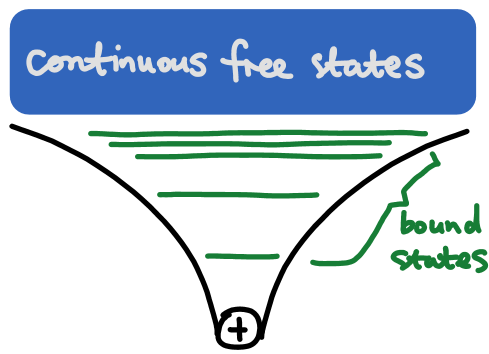
\includegraphics[width=0.3\textwidth]{bound_free_states_H}}
\textbox{Bound states in general\index{bound state}}{
    Here we only calculated the case of square potential. And only considered infinite potential well in details. However, the qualitative conclusion is general: If the quantum state does not have enough energy to reach infinity, then the state is a bound state localized in or close to the well. The energy of the state can only take discrete values. There exists a lowest energy state known as the ground state. For example, a nuclei has positive charge and creates a set of bound states that electrons can occupy.
}

\textbox{Optional: Two potential barriers together and resonant tunneling\index{potential: double barrier}\index{resonant tunneling}}{
    What \marginnote{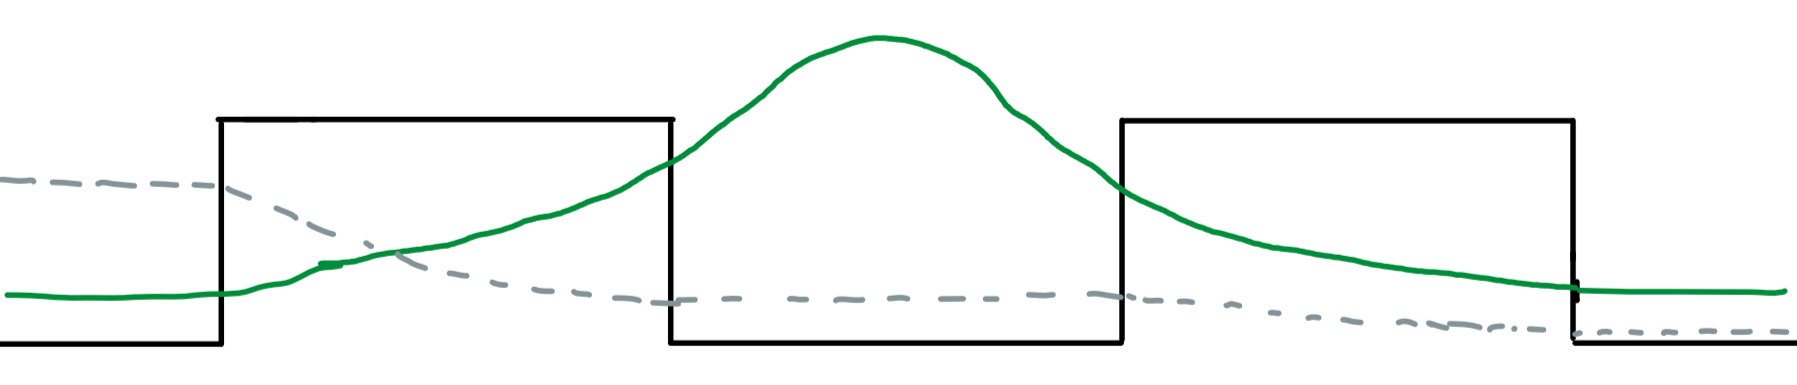
\includegraphics[width=0.4\textwidth]{p_resonance}}
    about putting two identical potential barriers together? We then have a potential well in between two potential barriers. The potential well can hold bound states in it.

    Consider the tunneling problem with such double barrier. Usually, we get double exponential suppression factors. Thus there is doubly small chance to tunnel through double barrier as expected. The situation is illustrated by the gray dashed line in the figure.

    However, if we fine-tune the incoming energy to coincide with a bound state energy, then the gray dashed line is not a correct boundary condition for a bound state (for a bound state, both sides should exponentially decay) thus cannot be right. Rather, there is no exponential suppression factor for such tunneling. This situation is known as resonant tunneling. 
    \tcblower
    This explains 王二's enhanced tunneling rate (item \ref{item:resonant-tunneling} at the beginning of this part) if we consider the front and back wall as two potential barriers and 王二's incoming energy coincides with a bound state in the room.
}


\textbox{Optional: Two potential wells together and split of ground state\index{potential: double well}}{
    What \marginnote{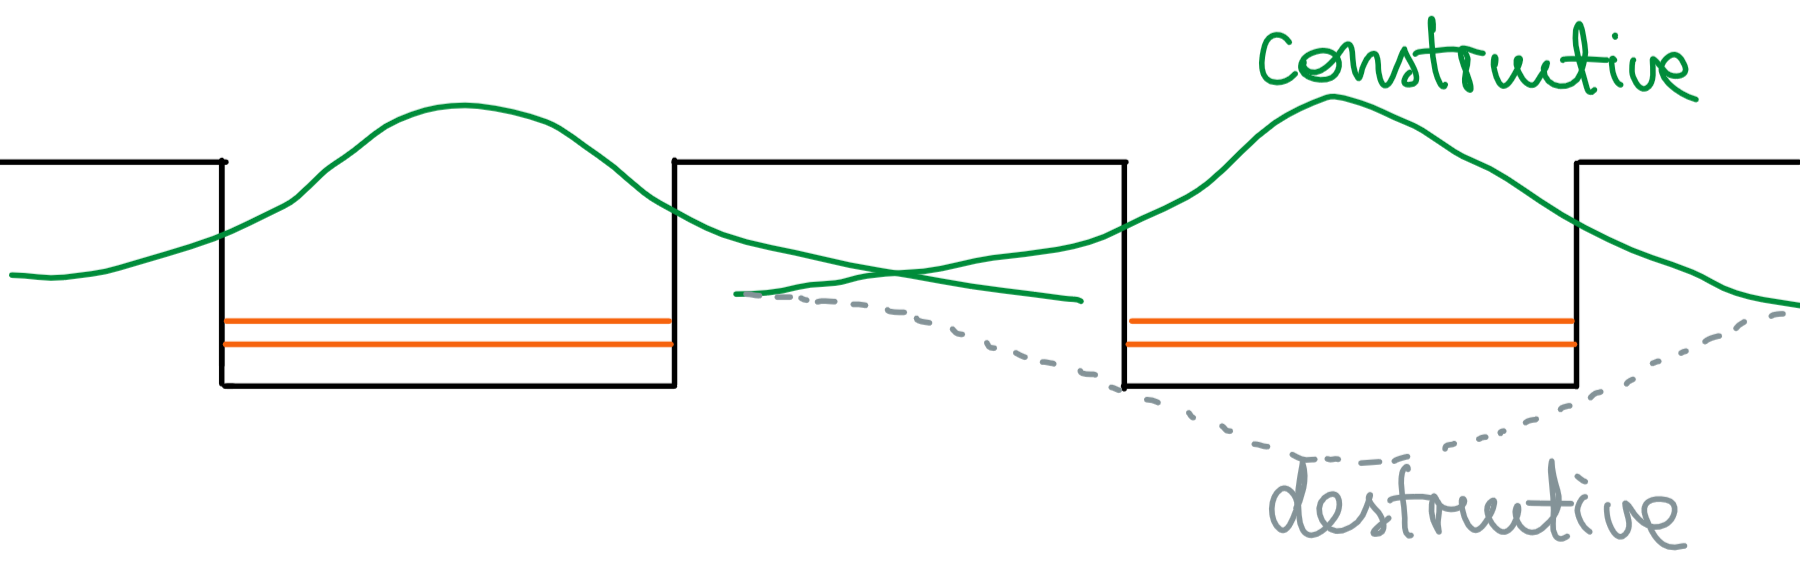
\includegraphics[width=0.4\textwidth]{p_double_well}}
    about putting two identical potential wells together (called ``double well'')? Each potential well has its own set of bound states. Do the two set of bound states affect each other?

    For definiteness, let us call the ground state of the left well $\psi_L$, and the ground state of the right well $\psi_R$. Both of them have energy $E$. Are $\psi_L$ and $\psi_R$ the lowest energy state of the system?

    Due to linearity of quantum mechanics, we know that the superpositions $\psi_\pm=(\psi_L \pm\psi_R)/\sqrt 2$ are also solutions of the Schr{\"o}dinger equation. In fact $\psi_+$ has slightly lower energy than $E$ because the wave function takes slightly larger value in the middle barrier (constructive interference), which makes the position of the particle less certain. Similarly, $\psi_-$ has slightly higher energy due to destructive interference. Thus the original ground state splits into two states, with $\psi_+$ the true ground state of the theory.
}


\textbox{Optional: Infinite potential wells together and the band theory\index{potential:periodic}\index{energy band}}{
    What \marginnote{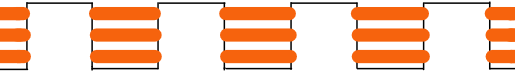
\includegraphics[width=0.4\textwidth]{p_periodic}} about putting infinitely many identical potential barriers (or wells) together? We get a periodic potential. From the experience of double well, the sign of each local ground state (of an individual well) can make constructive or destructive interferences. There are infinitely many choices. Thus the original ground state splits into an infinite number of states. These states form a continuous band.

    The 
    \mtextbox{Quantum mechanics in your phone}{
        You should appreciate quantum mechanics for allowing you to have a cell phone. Indeed, the CPU of your phone is doing classical computing, not quantum computing yet. But the logical gates of a modern classical computer is based on semi-conductors, and thus the band theory of solid state physics. Without quantum mechanics, we cannot understand these theories and there is nothing to guide us for making transistors from semi-conductors.
    }
    particle energy has to be within the band. And resonant tunneling happens and the quanta can freely travel through potential barriers without suppression.

    Here we are talking about the ground state. But for other higher energy states, the same argument applies that the bound state energies are broadened into continuous bands (illustrated by the orange thick lines in the figure).
    
    \tcblower

    The infinite potential can be considered as a toy model of a solid. The potential wells are those made by atoms, and the quanta being studied are the electrons. In solid, the energy of the active electrons is determined by statistical physics and the nature of the solid (the ``Fermi energy'' at low temperature). If the electrons can move in the band, the solid can conduct electric current and thus is a conductor. If the conducting band is fully occupied, the solid is an insulator. The case in between is known as semi-conductor. 
}

\section{Identical Particles}

At the beginning of this part, item \ref{item:identical} of 王二's adventure is that she fails to distinguish an electron from another. In the classical world, we can distinguish persons. Why this fails to work in 王二's quantum adventure?

\textbox{The classical ways of distinguishing particles all fail\index{identical particles}}{
    Classically, how we distinguish two persons?
    \tenum{
        \item Intrinsic identifications: Classically, two persons look different. However, for microscropic particles, this fails to work. Because:
        \titem{
            \item Elementary particles: We have only discovered finite types of elementary particles (labeled by mass, spin and charge). Two particles of the same type have the same intrinsic features. For examples, you cannot find any difference between two electrons.
            \item Composite particles (such as atoms): They are bound states. Bound state energies are discrete. For example, if two hydrogen atoms are both in their ground states, or first excited states, we cannot find any difference between the two atoms.
        }
        \item Extrinsic identification: Classically, two persons are separate. We can follow their trajectories to distinguish them. 如果王三在,周十一 is in New York, it's easy to figure out whom is whom even if they look alike. 

        However, quantum particles can never be in totally different positions. Fundamentally, what separate quantum particles are potential wells. Quantum tunneling tells that the wave function of two particles, say electrons, will always overlap, though the amount may be extremely small. Two electrons are never completely separated.
    }
    \tcblower
    Those failure of distinguishing quantum particles lead to a fundamental principle of quantum mechanics: the existence of identical particles.
}

\textbox{Classification of quantum particles\index{bosons}\index{fermions}}{
    To make use of the identical particle postulate, we need a wave function to describe at least two particles. The two-particle wave function $\Psi(x_1, x_2, t)$ means that the probability to find one particle at $(x_1, x_1 +dx_1)$ and the other particle at $(x_2, x_2+dx_2)$ is $|\Psi(x_1, x_2, t)|^2 dx_1 dx_2$.

    Since the two particles are identical, we should have $|\Psi(x_1, x_2, t)|^2 = |\Psi(x_2, x_1, t)|^2$. Otherwise, we can tell the difference of the two particles by noticing the probability difference that the two particles can be found.\marginnote{Imagine one twin likes more to go to a coffee shop and the other twin likes more to go to a bookstore. You can then distinguish them in a statistical sense, and they are no longer identical.} Thus, $\Psi(x_1, x_2, t)$ and $\Psi(x_2, x_1, t)$ differ at most by 
    \begin{align}
        \Psi(x_2, x_1, t) = e^{i\alpha} \Psi(x_1, x_2, t)~,
    \end{align}
    where $\alpha$ is a real number. Mathematically, this implies (since $x_1$ and $x_2$ are just labels that can be swapped)
    \begin{align}
        \Psi(x_1, x_2, t) = e^{i\alpha} \Psi(x_2, x_1, t)~.
    \end{align}
    Thus, $e^{i\alpha} = \pm 1$. The multi-particle wave functions are either symmetric or asymmetric under interchange of particles.


    \tcblower
    There are thus two kinds of multi-particle wave functions which satisfies the identical particle postulate:
    \titem{
        \item Symmetric wave functions with $\Psi(x_1, x_2, t) = \Psi(x_2, x_1, t)$. The particles described by such wave functions are called bosons. For elementary particles, bosons represents the forces of nature, for example, photons and gravitons. 
        \item Anti-symmetric wave functions with $\Psi(x_1, x_2, t) = - \Psi(x_2, x_1, t)$. The particles described by such wave functions are called fermions. For elementary particles, fermions represents the buliding blocks of matter, for example, electrons and quarks.
    }
}

\textbox{Pauli's exclusion principle\index{Pauli's exclusion principle}}{
    For fermions, because of the anti-symmetry of the wave function, the fermions cannot be in the same state. This is because, if two fermions were in the same state, then

    $\Psi(x_1, x_2, t) = \Psi(x_2, x_1, t)$. Considering the definition of fermions, $\Psi(x_1, x_2, t) = -\Psi(x_2, x_1, t)$, we get $\Psi(x_1, x_2, t)=0$ and thus such systems do not exist.

    This is why in a multi-electron atom, electrons do not only occupy the lowest energy states, but also other states if some electrons have already occupied the lowest energy states.
}

\section{Epilogue: Summary and What's Next} \label{sec:epilogue-qm}

In the journey of constructing the theory of quantum mechanics, we have met many difficulties. The difficulties are resolved sometimes by applying what we know; and sometimes by introducing new postulates. Now, let us summarize the postulates that we really have to introduce.

\needspace{0.2\textheight}
\textbox{Summary of fundamental postulates of quantum mechanics}{
    \tenum{
        \item The superposition principle of $\psi(\mathbf{x},t)$: the world is linear.
        \item Momentum can be represented by an operator $\mathbf{\hat p} = -i\hbar \mathbf{\partial_x}$.
        \item A measurement
        \marginnote{Recall that if the observable take discrete values, the corresponding decomposition is
        $$ \psi(\mathbf{x}) = \sum_i c_i \psi_{\lambda_i}(\mathbf{x}) $$ and the probability to get $\lambda_i$ is $|c_i|^2$
        }
        is represented by a Hermitian operator $\hat O$. The operator $\hat O$ defines a complete set of eigenstates $\hat O \psi_\lambda(\mathbf{x}) = \lambda \psi_\lambda (\mathbf{x})$. The state to be measured $\psi(\mathbf{x})$ can be expended by these eigenstates as $\psi(\mathbf{x}) = \int c(\lambda) \psi_\lambda ~ d\lambda$. The probability density to get value $\lambda$ from the measurement is $|c(\lambda)|^2$ and the state collapses to $\psi_\lambda (\mathbf{x})$ after the measurement. 
        \item The wave function obeys the Schr{\"o}dinger equation
        \begin{align}
            i\hbar\partial_t \psi(\mathbf{x}, t) = \hat H \psi(\mathbf{x}, t)~,
            \qquad \hat H \equiv  -\frac{\hbar^2\nabla^2}{2m} + V(\mathbf{x})
        \end{align}
        \item Particles can be identical in quantum mechanics.
    }
    \tcblower
    These postulates do not look as simple as those of relativity. This is why it took decades for the sages of the past century to understand the principles of quantum mechanics. Fortunately, once we have understood and accepted these postulates, the quantum world works elegantly and amazingly. 
}

We have discussed how these postulates are natural guesses inspired from experiments, and explored the consequences of these postulates. Having that said, we do not know what ``really happens'' in quantum mechanics, especially when a measurement is made. Let me mention it further here:

\textbox{The Schr{\"o}dinger's cat: how to understand superposition and measurements?\index{Schr{\"o}dinger's cat}}{
    Traditionally, the Copenhagen (a city where a large part of quantum mechanics is developed) interpretation encourage ``shut up and calculate.'' However, we may not like to shut up at a thought experiment known as the Schr{\"o}dinger's cat:

    \begin{center}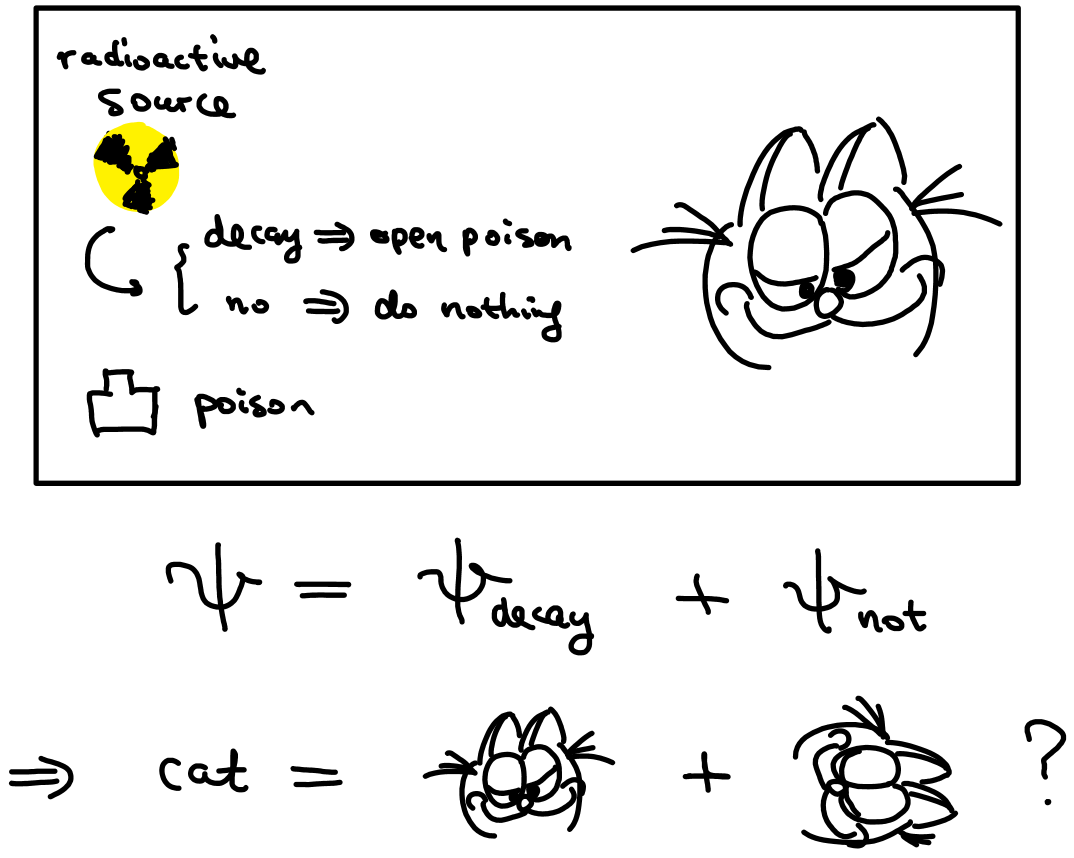
\includegraphics[width=0.5\textwidth]{garfield}\end{center}

    If a quantum process controls whether a bottle of poison opens. And we put the quantum generator, bottle of poison and a cat in a box. Before we open the box and measure the state, what happens to the cat? Is the cat in a superposition of alive and death?

    Unfortunately, no firm answer can be given at the moment. The answers differ in different interpretations of quantum mechanics. In some interpretations, one may even so crazy to let both the alive and dead cat live in parallel universes after the measurement, and we are only in one of them!
}

\textbox{Further reading about the content}{
    \titem{
        \item To learn more, the best way is to read the first a few sections of a proper quantum mechanics book. For example, Griffiths, \href{https://www.amazon.com/Introduction-Quantum-Mechanics-David-Griffiths/dp/0131118927}{Introduction to Quantum Mechanics}, or Allan Adams, Matthew Evans, and Barton Zwiebach
        \href{https://ocw.mit.edu/courses/physics/8-04-quantum-physics-i-spring-2013/}{MIT Open Course on Quantum Mechanics} (with videos). 
        \item \href{https://www.amazon.com/Principles-Quantum-Mechanics-P-Dirac/dp/1607965607/ref=sr_1_1?ie=UTF8&qid=1538490635&sr=8-1&keywords=the+principle+of+quantum+mechanics+dirac}{The Principles of Quantum Mechanics} by Dirac, though a bit old, is still an excellent introduction.
        \item Some other famous books include Shanka, \href{https://www.amazon.com/Principles-Quantum-Mechanics-2nd-Shankar/dp/0306447908/ref=sr_1_10?s=books&ie=UTF8&qid=1504075898&sr=1-10&keywords=quantum+mechanics}{Principles of Quantum Mechanics}, Sakuri, \href{https://www.amazon.com/Modern-Quantum-Mechanics-Revised-Sakurai/dp/0201539292/ref=sr_1_2?s=books&ie=UTF8&qid=1504076022&sr=1-2&keywords=quantum+mechanics+modern}{Modern Quantum Mechanics}.
        \item For the developments of quantum mechanics, there is a popular science book in Chinese: Cao, \href{https://book.douban.com/subject/1467022/}{Does God Play Dice}.
    }
}

\textbox{What happens next in a university physics program?}{
    \titem{
        \item Quantum mechanics and advanced quantum mechanics. What I have covered is really a starting point and you need to learn a proper course. You need to learn the algebra of matrices, the quantum harmonic oscillator, angular momentum, approximation methods, and so on.
        \item Atom physics, solid state physics and material science. The explanation of matter is all based on quantum mechanics.
        \item Quantum field theory. This is how quantum mechanics works with special relativity.
    }
}

\section{Exercises}

\textbox{E\wref{sec:photon}.1 Compton effect}{
    Derive the wavelength shift \eqref{eq:compton} for the Compton effect.
} 

\textbox{E\wref{sec:uncertainty}.1 Time evolution of the eigenstates}{
    What is the form of position eigenstates (quantum states with definite position) and momentum eigenstates for a freely moving particle? At the next moment in time (without measurement or interaction), are they still position and momentum eigenstates?
}

\textbox{E\wref{sec:uncertainty}.2 Uncertainty of the Gaussian wave packet}{
    Compute $\sigma_x$ and $\sigma_p$ of the Gaussian wave packet \eqref{eq:guassian_x}. Show that the uncertainty principle is satisfied in a saturated way.
}

\textbox{E\wref{sec:uncertainty}.3 Commutation relations}{
    If $\psi_q(x)$ is an eigenstate of $x$ with eigenvalue $q$. Can $\psi_q(x)$ also an eigenstate of $\hat p$? Let us answer this question in different ways:
    \titem{
        \item Physically: show that if $\psi_q(x)$ is at the same time eigenstate of $x$ and $\hat p$, then the uncertainity principle is violated.
        \item Mathematically: Show that $\hat p (x \psi_q(x)) \neq x (\hat p \psi_q(x))$. Use this observation to prove that $x$ and $\hat p$ do not share eigenstates.
    }
}

\textbox{E\wref{sec:schro-all}.1 Time-dependent scattering on a potential barrier}{

    Consider a particle moving towards a barrier-shaped potential, and the incoming energy is lower than the height of the barrier (i.e. the potential energy on the barrier is higher than the total energy of the particle).

    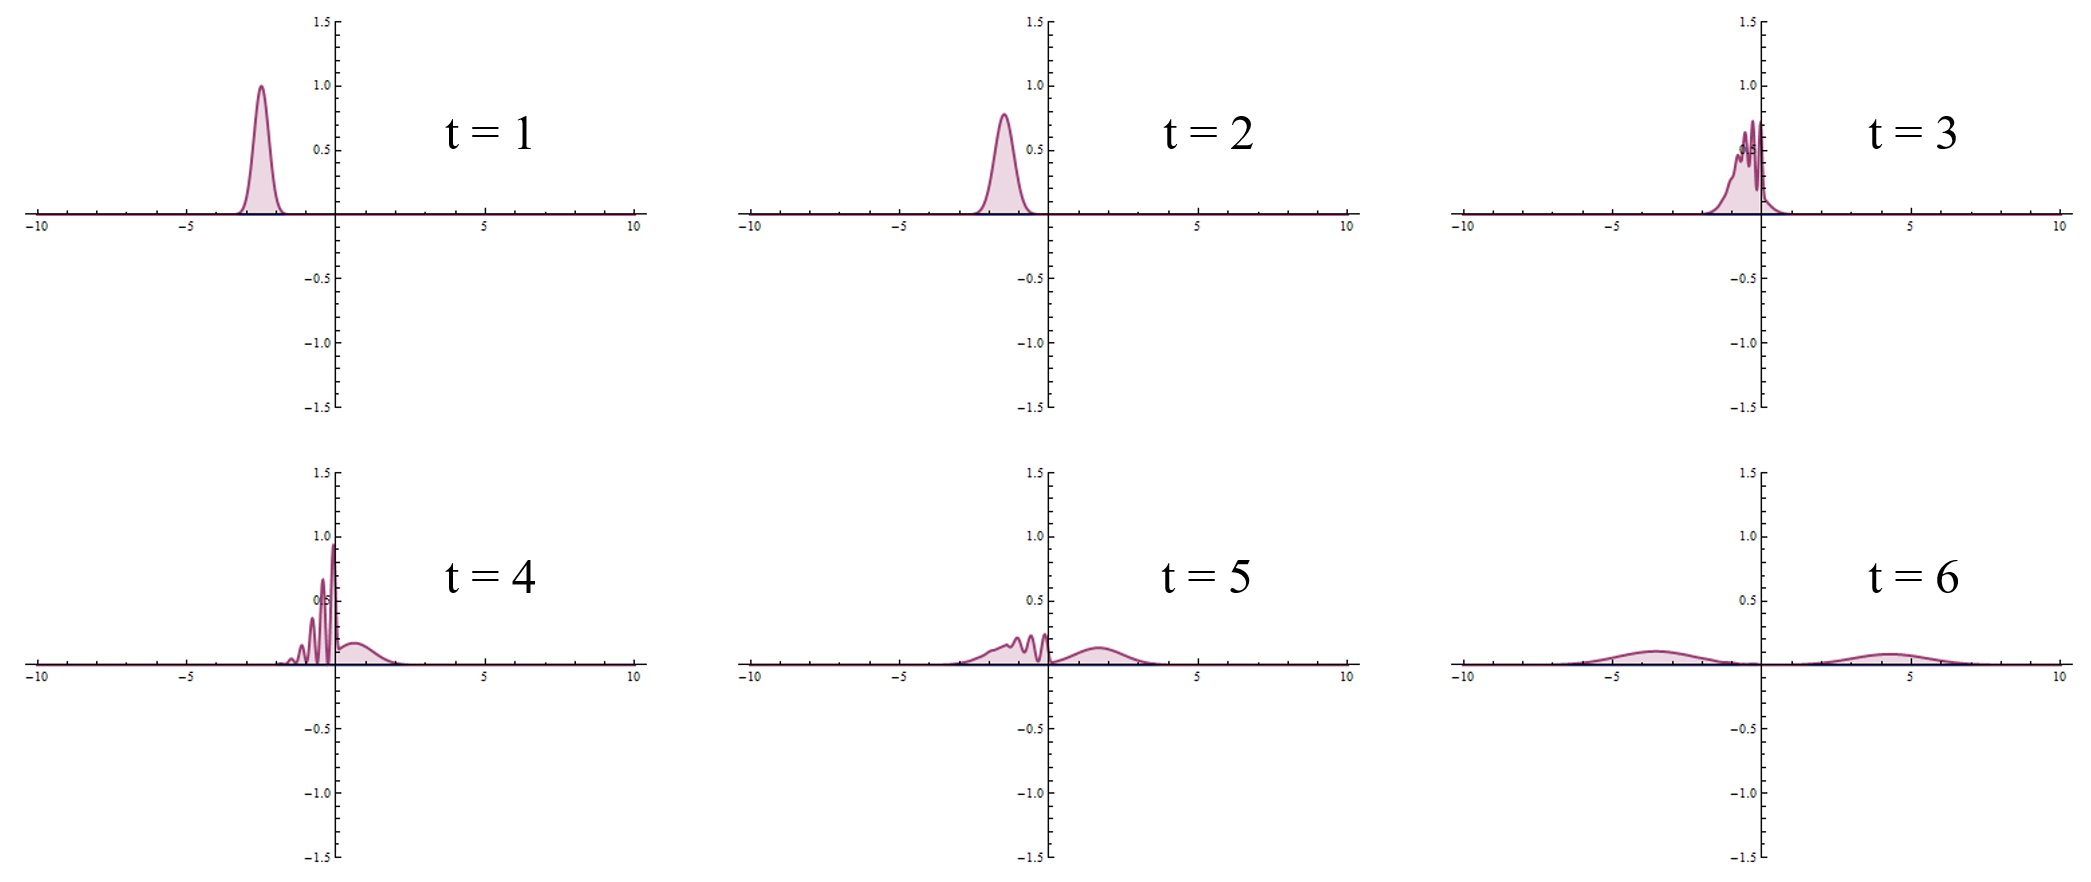
\includegraphics[width=\textwidth]{tt}

    \titem{
        \item Classically, can the particle pass to the other side of the barrier? Why?
        \item Quantum mechanically, can the particle pass to the other side of the barrier? Why? Explain it both in terms of continuity of the wave function, and energy conservation.
        \item Some ripples are observed in the figure below (snapshots of the probability density of the particle). Explain the ripples qualitatively.
    }
}


\textbox{E\wref{sec:schro-all}.2 Scattering on a potential barrier: math and interpretations}{
    \titem{
        \item Derive the transmission amplitude $E$ using $A$ for a potential barrier.
        \item Show that the relations between $A$, $B$ and $E$ conserves probability.
        \item Show that $E$ is exponentially suppressed if $E<V_2$. Find the exponential factor.
    }
}

\textbox{E\wref{sec:schro-all}.3 Bound states}{
    Consider bound states in a square potential well.
    \titem{
        \item Count number of free parameters and number of constraint conditions, to show that energy needs to be quantized for bound states.
        \item When measuring the energy of a superposition of bound states with different energies, must the outcome of the measured energy quantized?
        \item Keep the depth of the potential well fixed and increase the width. Shall the number of bound states increase or decrease? Why?
    }
}

\printindex

\end{document} 